\documentclass[12pt]{report}
\usepackage[utf8]{inputenc}
\usepackage[english]{babel}
\usepackage{microtype}
\usepackage{libertine}
\usepackage{amsmath,amsthm}
\usepackage[varg]{newtxmath}
\usepackage{setspace,graphicx,epstopdf}
\usepackage{marginnote,datetime,url,enumitem,subfigure,rotating}
\usepackage{multirow}
\usepackage{xfrac}
\usepackage[openlevel=3]{bookmark}
\usepackage[tikz]{bclogo}
\usepackage{enumitem}

\setcounter{tocdepth}{2}

\def\D{\mathrm{d}}

\setlength{\parindent}{0ex}
\setlength{\parskip}{1em}%Espacement des par

\setlist[itemize]{topsep=-2pt}

\newcommand{\smalltodo}[2][] {\todo[caption={#2}, size=\scriptsize,%
fancyline, #1]{\begin{spacing}{.5}#2\end{spacing}}}
\newcommand{\rhs}[2][]{\smalltodo[color=green!30,#1]{{\bf PS:} #2}}

\newcommand{\E}[1]{\operatorname{E}\left[#1\right]}
\newcommand{\Et}[1]{\operatorname{E}_t\left[#1\right]}
\newcommand{\V}[1]{\operatorname{Var}\left[#1\right]}
\newcommand{\cov}[1]{\operatorname{Cov}\left(#1\right)}
\newcommand{\covt}[1]{\operatorname{Cov}_t\left(#1\right)}
\newcommand{\avg}[2]{\frac{#1}{#2} \sum_{i=#1}^{#2}}
\def\D{\mathrm{d}}


\begin{document}

\date{}
\title{\textbf{\huge{ECON7751 - Macroeconomic Theory II}}\\ \textit{Lecture Notes from Susanto Basu's lectures}}
\author{Paul Anthony Sarkis\\ Boston College} 
 
\maketitle

\tableofcontents

\chapter{Consumption Theory}

This chapter investigates the theory of consumption, or in other words, how agents choose the level of consumption based on their preferences subject to budget constraints. The introduction of the chapter looks at a simple two-period model and introduces the main topics of consumption theory. The following sections will look deeper into these concepts by analyzing consumer decisions under certainty and uncertainty for an infinite horizon.

\section{Introduction: the Fisher model}

\subsection{Preferences of the consumer}

In consumption theory, we assume that any household has preferences defined over a sequence of consumption levels, for each period in time. To start, we will consider the case of two-periods (Fisher model). This means that a consumer will choose two consumption levels ($c_t$ and $c_{t+1}$) to satisfy best his preferences.

A household has an instantaneous utility function $u(c)$ representing his preferences at each point in time. We typically assume that $u(\cdot)$ is an increasing concave function. The lifetime utility of any household will be assumed to be the net present value of every period's utility level. In order to discount utility, we assume the household has a subjective rate of time preference, denoted $\rho$, yielding the discount rate $\frac{1}{1+\rho}$. Already we can see a link between $\rho$ and the "patience" of the household. If $\rho$ is high, then the discount factor is low, future utility is not very important: the household is impatient. When $\rho$ is low, the discount factor is high: the household is patient.

In the two-period case, we define lifetime utility as: $$U(c_t, c_{t+1}) = u(c_t) + \frac{1}{1+\rho} u(c_{t+1}) $$ This form of utility is called time-separable since any variation of consumption affects only utility in that period. Note that sometimes we will use $\beta$ to denote the discount factor.

\subsection{Market structure}

The consumer faces two markets in this setting, the goods market, in which he buys consumption goods ($c$) at a normalized price of $1$, and an asset market, in which he buys assets that yield a return in the next period. The price of the asset is determined by its return in the next period, denoted $r$. For now, we assume that the consumer is a price-taker in both markets, meaning that he does not internalize the effects of his consumption on prices (the price of consumption and assets are fixed).

The consumer also gets an income for labor (fixed in this setting), denoted as $y$. He gets a wage in both periods.

\subsection{Budget constraint}

In order to solve the model, we have to make sure that the consumer can only buy with what he has in his budget. Approaching this setting with game theory, we can be sure that in the last period, the consumer will spend all his assets and his income in consumption (he has no incentive to save because he will not get the returns next period). Hence, in the second period, he consumes his income and the value of his assets saved in the first period: $$c_{t+1} = y_{t+1} + (1+r)a_{t+1} $$ In the first period, he can choose to either consume or save his income (assuming he has no initial wealth). This gives the following budget constraint: $$c_t + a_{t+1} = y_t $$
We see that both constraints must be satisfied in each period, and that they are linked by a variable: savings of the first period, $a_{t+1}$. This fact helps us writing both constraints as a single, inter-temporal constraint: $$c_t + \frac{1}{1+r}c_{t+1} = y_t + \frac{1}{1+r}y_{t+1} $$ In words, this constraint also means that the net present value of consumption must be equal to the net present value of income (also called human wealth).

\subsection{Optimality}

We can now set up the consumer's problem and solve it: $$\max_{c_t, c_{t+1}} u(c_t) + \beta u(c_{t+1})\text{ s.t. } c_t + \frac{1}{1+r}c_{t+1} = y_t + \frac{1}{1+r}y_{t+1} $$ This problem must satisfy the following two FOCs:\begin{itemize}
\item $u'(c_t) - \lambda = 0$
\item $\beta u'(c_{t+1}) - \frac{1}{1+r}\lambda = 0$
\item[$\Rightarrow$] $u'(c_t) = \beta (1 + r) \cdot u'(c_{t+1})$
\end{itemize}

This last equation is called the Euler equation for consumption: it determines the path of consumption with respect to market parameters. This Euler equation can also be interpreted in a different way. Consider $u'(c_t)$ as the marginal utility of consumption in the first period, while $\beta (1 + r) \cdot u'(c_{t+1})$ is the marginal utility of consumption in the second period. We can describe the latter also as the marginal utility of saving in the first period: thus, the optimal path of consumption equates the marginal utility of consumption and savings.

An interesting result of this Euler equation is that the path of consumption is not determined by income ($y$ does not appear in the Euler equation), this means that income only defines the level of consumption (through the IBC). To see this clearly, consider the case when $\rho = r$, then $\beta = \frac{1}{1+r}$ and we have that Euler equation yields: $$u'(c_t) = u'(c_{t+1}) \Leftrightarrow c_t = c_{t+1} $$ regardless of what happens to income. This result is linked to a few hypotheses that we will try to let go of in the next sections. In particular, this is the case because consumers can borrow and lend freely, in a perfect financial market and also because there is no uncertainty with respect to interest rates, income, etc.

\subsection{Intertemporal-substitution and wealth effects}

In order to investigate comparative static, we will use a specific yet general enough utility function, a CES utility of the form: $u(c) = \frac{c^{1-\sigma}}{1-\sigma}$ which is $\ln(c)$ when $\sigma = 1$. Using this functional form, we can interpret $\sigma$ as the willingness to smooth consumption: the smaller $\sigma$ is, the more willing a consumer is to let their consumption vary over time. We can see that by actually solving the Euler equation. We know that $u'(c) = c^{-\sigma}$, thus: $$u'(c_t) = \beta (1 + r) \cdot u'(c_{t+1}) \Rightarrow \frac{c_{t+1}}{c_t} = \left(\frac{1+r}{1+\rho}\right)^{\frac{1}{\sigma}} $$ Here, the higher $\sigma$ is, the closer to 1 is the inter-temporal ratio of consumption, meaning that consumption will be almost equal at all periods.

Using a CES utility function allows us to derive a simple form for the inter-temporal elasticity of substitution (IES), denoted $\theta$. The IES is defined as: $$\theta(c) \equiv -\frac{u'(c)}{u''(c)c} = \frac{c^{-\sigma}}{-\sigma c^{-\sigma}} = \frac{1}{\sigma}$$ which is a constant for any level of consumption (giving the name CES).

The inter-temporal rate of substitution can give us interesting insight about how the consumption path reacts to changes in the interest rate. From the Euler equation, we already know that a higher $r$ implies a steeper consumption path ($c_{t+1}/c_t$ is greater). In fact, it seems logical since $1+r$ is in fact the relative price of $c_t$ in terms of $c_{t+1}$. Therefore, we could say that in general, a higher $r$ tends to increase savings.

However, analysis of an increase is not that simple because $r$ also determines the net present value of wealth and a higher $r$ would also mean lower wealth if the consumer is borrowing, higher wealth if he is lending, or nothing if he has no assets. One must consider these cases when looking at the effect of an increase in $r$.

Note: a log-utility function ($\sigma = 1$) means a one for one substitution of consumption between periods.

\section{Consumption under Certainty}

We have previously introduced the main objective of consumption theory, looking at consumption decisions with respect to income, interest rates, preferences, etc., but we did it in a very simplistic way. The next two sections are going to treat this topic in a more general way, yet leaving it simple enough. By simple enough, we mean that we still consider the consumer as a price-taker in markets, his labor decision is still fixed, and all functions are relatively well-behaved.

\subsection{Model}

A representative consumer seek to maximize lifetime utility by choosing an optimal path for consumption, subject to instantaneous budget constraints: $$\max_{\{C_t\}} U_t \equiv \sum_{s=0}^{\infty} \beta^{s} u(C_{t+s}) \text{ s.t. } C_{t+s} + A_{t+s+1} = (1+r)A_{t+s} + Y_{t+s} \quad \forall s \geq 0 $$ Recall that the utility function used above is additively time-separable.

In this model, $A_t$, the asset holdings, is a state variable. We call it this way because it summarizes all past decisions on consumption, given the past realizations of income (since not consuming increases $A$).

The income, $Y_t$, is an exogenous variable: it is not linked to any decision and it fluctuates freely. Even though the same things can be said of $\beta$ and $r$, we call these variables the parameters of the model, since they do not move in time.

Finally, consumption $C_t$ is the choice (or control) variable of the model: the variable used to solve the model. Note that controlling $C_t$ also means controlling $A_{t+1}$ because of the instantaneous budget constraint.

\subsection{Optimality}

Since choosing $C_t$ and $A_{t+1}$ is the same thing, we can solve the model by replacing $C_t$ by its constraint expressed in assets holdings terms and solve it. $$\max_{\{A_{t+1}\}} U_t \equiv \sum_{s=0}^{\infty} \beta^{s} u((1+r)A_{t+s} + Y_{t+s} - A_{t+s+1}) $$ which yields the following FOCs, for all $s$: $$ - u'(C_{t+s}) +\beta(1+r)u'(C_{t+s+1}) = 0 $$ which is exactly the Euler equation that we found in the two-period case. Note that because this equation holds for any $s\geq 0$, we can replace $u'(C_{t+s+1})$ by any further condition, meaning that at any point in time, the optimal path is set in stone from the first period. We say that the consumption decision is time consistent.

\subsection{Explicit solution: polynomial utility case}

In order to look at the consequences of such a model, let's assume a polynomial utility function representing the consumer's preferences: $$u(C_t) \equiv \alpha_0 C_t - \frac{\alpha_1}{2} C_t^2 $$ Further, we assume that $\beta$ and $r$ are defined such that $\beta(1+r)=1$ or equivalently, we assume that $\rho = r$.

Recall the Euler equation: $u'(C_{t+s}) = \beta(1+r)u'(C_{t+s+1})$, now we can rewrite it as: $$\alpha_0 - \alpha_1C_{t+s} = \alpha_0 - \alpha_1C_{t+s+1} $$ $$\Leftrightarrow C_{t+s} = C_{t+s+1} $$ This result implies that the optimal decision for the consumer is to perfectly smooth consumption: exactly what we found in the previous section with the CES utility function.

Now this equation, while powerful, does not solve the model. In fact, the solution to any dynamic model is an expression that links control variables to state and exogenous variables. In our case, we need to find the expression of $C_t$ in terms of $A_t$, $Y_t$, $r$ and $\beta$.

To do that, start with the instantaneous budget constraint: $$C_t + A_{t+1} = (1+r)A_t + Y_t $$ and write in terms of $A_t$: $$A_t = \frac{1}{1+r}A_{t+1} +\frac{1}{1+r}C_t - \frac{1}{1+r}Y_t $$ Since this instantaneous budget constraint holds for any period, we can write: $$A_{t+1} = \frac{1}{1+r}A_{t+2} +\frac{1}{1+r}C_{t+1} - \frac{1}{1+r}Y_{t+1} $$ and replace it in the previous budget constraint: $$A_t = \frac{1}{1+r}\left[\frac{1}{1+r}A_{t+2} +\frac{1}{1+r}C_{t+1} - \frac{1}{1+r}Y_{t+1}\right] +\frac{1}{1+r}C_t - \frac{1}{1+r}Y_t $$ and we get: $$A_t = \lim_{T\to\infty}\frac{1}{(1+r)^T}A_T + \frac{1}{1+r}\sum_{s=0}^{\infty}\frac{1}{(1+r)^s}(C_{t+s} - Y_{t+s}) $$ The first term seems scary but if you look at it closely you can see how to simplify it. Indeed, the term represents the net present value of the consumer's assets at the infinite horizon. This value cannot be negative, because of the no-Ponzi-game condition (else, the consumer would roll over debt ad infinitum to consume more and more). Moreover, the value cannot be positive (again, by a game-theoretic approach, any rational agent would consume all his wealth in the last period). Then, it must be that the term is equal to 0. We are then left with two terms: the net present value of consumption, and the net present value of income (human wealth). We can write: $$A_t + H_t = \frac{1}{1+r}\sum_{s=0}^{\infty}\frac{1}{(1+r)^s}C_{t+s} $$ Using the Euler equation of earlier, we know that consumption is perfectly smooth, meaning that we can write $C_t$ for any $C_{t+s}$. This allow us to simplify or equation to: $$A_t + H_t = \frac{1}{1+r}C_{t} \frac{1}{1 - \frac{1}{1+r}} $$ $$\Leftrightarrow A_t + H_t = \frac{C_{t}}{r} $$ $$\Leftrightarrow r(A_t + H_t) = C_{t}$$ In the same way, if we assume that $Y_t$ is constant for all periods, we can write the exact definition of consumption as: $$C_t = rA_t + Y_t $$ which replaced in the budget constraint gives $A_t = A_{t+1}$: wealth is constant over time.

\section{Consumption under Uncertainty}

\subsection{Model}

Again, we use a representative household in an economy such that he can borrow and lend freely (no transaction costs) at a fixed interest rate $r$. The horizon is infinite (Ramsey model) so as before we get:$$\max_{C_t} \Et{\sum_{s=0}^{\infty}\beta^s U(C_{t+s})} \text{ s.t. } C_{t+s} + A_{t+s+1} = (1+r)A_{t+s} + Y_{t+s} $$

However, this time we assume that consumers do not know future realizations of variables. In particular, we say that the variable $Y_t$ (the only variable that consumers have no control on) is stochastic. Agents know the probability distribution of $Y_t$ (its stochastic process). Therefore, in order to solve the problem, we assume that consumers have rational expectations.

\subsubsection{Rational Expectations}

Agents formulate expectations in such a way that their subjective probability distribution of economic variables (conditional on the available information) coincides with the objective probability distribution of the same variable (according to a measure of the state of nature) in an equilibrium. This means that agents have perfect foresight, under uncertainty.

As we've seen above, we represent these expectations by using the notation $\Et{\cdot}\equiv \E{\cdot\vert I_t}$, the  expectation of any variable, conditional on the information set at time $t$.

Rational expectations have some interesting properties:\begin{itemize}
\item No systematic bias: $\Et{C_{t+1} - \Et{C_{t+1}}} = \Et{\varepsilon_{t+1}} = 0$
\item No autocorrelated bias: $\cov{\varepsilon_{t+s},\varepsilon_{t}} = 0$ for all $s\neq 0 $ 
\item Law of iterated expectations: $\Et{E_{t+s}\left[X_{t+v}\right]} = \Et{X_{t+v}}$ for all $v\geq s\geq 0$ 
\end{itemize}

\subsubsection{Optimal path à la Basu}

This time we use the method of perturbation (Basu's favorite)  in order to find the optimal path. Let $\delta > 0$ be a variation so small in level that $U'(x + \delta) \approx (\delta)U'(x)$. Now, assuming you are on the optimal path, consider $\delta$ to be an amount that you choose not to consume today in order to consume it tomorrow. That is, you save $\delta$ more today and get to consume $\delta (1+r)$ more on next period, on in other words, you take off from the optimal path. Because this perturbation takes you out of the optimal path, the reallocation of $\delta$ has to incur a loss in utility. Therefore we get: $$(-\delta)U'(C_t) + \Et{(\delta)\frac{1+r}{1+\rho}U'(C_{t+1})} \leq 0 $$  In the same manner, a positive perturbation of $\delta$ will also cause a loss in utility, hence: $$(\delta)U'(C_t) + \Et{(-\delta)\frac{1+r}{1+\rho}U'(C_{t+1})} \leq 0 $$ You can clearly see that both equations are perfect oppposites of each other, implying that: $$ - U'(C_t) + \Et{\frac{1+r}{1+\rho}U'(C_{t+1})} = 0 $$ This is the Euler equation for consumption, under uncertainty.

\subsubsection{Consumption as a random walk}

In order to let the model give us more insight on consumer behavior, we will have to make some assumptions. First, we impose a restriction that $r_t = r$, meaning that the interest rate is fixed. This will of course be true is the steady-state. Second, we also assume that this interest rate is equal to $\rho$, or equivalently, that $\beta(1+r) = 1$, which will also be satisfied in equilibrium. These two assumptions yield a simplified version of the Euler equation: $$ - U'(C_t) + \Et{U'(C_{t+1})} = 0 $$
$$\Leftrightarrow U'(C_t) = \Et{U'(C_{t+1})} $$ This only gives one (not very informative) piece of information: the optimizing consumer will choose a path of consumption so that his expected marginal utility is the same for all period: he smooths consumption over time.

In order to simplify further the previous Euler equation, Hall (1978) assumes that utility follows a quadratic form with a satiation point at $\bar C$. If $\bar C$ is far enough from the typical level of consumption, we have that $U(\cdot)$ is concave.

In particular, let $U(C_t) = -(\bar C - C_t)^2$. Then, \begin{align*}
U'(C_t) & = \Et{U'(C_{t+1})} \\
2(\bar C - C_t) & = \Et{2(\bar C - C_{t+1})} \\
C_t & = \Et{C_{t+1}}\\
C_{t+1} & = C_t + \varepsilon_{t+1} \text{ where } \Et{\varepsilon_{t+1}} = 0
\end{align*} This result is one of the most important in consumption theory. Note that it resembles closely the two previous results implying perfect smoothness of consumption, this time adding the fact that income is uncertain. This result has three main implications:\begin{enumerate}
\item Current consumption alone is the best predictor of future consumption. This comes from the fact that the error term is i.i.d. with mean zero.
\item Changes in consumption are ex-ante unpredictable. In fact, if you look at $\Et{C_{t+1} - C_t}$, you get: $$ \Et{C_{t+1}} - C_t = 0 $$
\item Consumption follows a random walk. This is the basic result that comes from the form of the equation.
\end{enumerate}

These consequences will be tested in a follow-up discussion on the permanent income hypothesis which includes all these results in an interesting and useful narrative.

\subsubsection{Explicit solution}

Now that we know what variations in the consumption will look like (we know that consumers will smooth), we are interested in the actual consumption function.

Starting from the budget constraint, we have that: $$A_{t+1} = (1+r)A_t + Y_t - C_t $$ where all variables are known at time $t$ (remember that $A_{t+1}$ is the decision made at time $t$); we rewrite this equation as a forward looking equation as: $$A_t = \frac{1}{1+r}A_{t+1} + \frac{1}{1+r}C_t - \frac{1}{1+r}Y_t $$ which must hold at all time, in particular at time $t+1$: $$A_{t+1} = \frac{1}{1+r}A_{t+2} + \frac{1}{1+r}C_{t+1} - \frac{1}{1+r}Y_{t+1} $$ Now we know $A_{t+1}$, but we do not know anything about the other variables. We can nevertheless use rational expectations to clear things out: $$A_{t+1} = \frac{1}{1+r}\Et{A_{t+2}} + \frac{1}{1+r}\Et{C_{t+1}} - \frac{1}{1+r}\Et{Y_{t+1}} $$ Replacing this last equation in the contemporaneous budget constraint yields: $$A_t = \frac{1}{1+r}\left[\frac{1}{1+r}\Et{A_{t+2}} + \frac{1}{1+r}\Et{C_{t+1}} - \frac{1}{1+r}\Et{Y_{t+1}}\right] + \frac{1}{1+r}C_t - \frac{1}{1+r}Y_t $$ $$\Leftrightarrow A_t = \frac{1}{(1+r)^2}\Et{A_{t+2}} + \frac{1}{(1+r)^2}\Et{C_{t+1}} - \frac{1}{(1+r)^2}\Et{Y_{t+1}} + \frac{1}{1+r}C_t - \frac{1}{1+r}Y_t $$ This process can be repeated many times, until the limit: $$A_t = \lim_{T\to\infty} \frac{1}{(1+r)^T}\Et{A_T} + \sum_{s=0}^{T} \frac{1}{(1+r)^{s+1}}\Et{C_{t+s} - Y_{t+s}} $$ Using the no-Ponzi game condition, we can restrict the value of assets to be equal to zero at the limit. Adding the expected NPV of income of both sides, we get that the expected NPV of consumption is equal to the assets holdings at time $t$ plus the expected NPV of labor (or human wealth): $$ \frac{1}{1+r} \Et{\sum_{s=0}^{T} \frac{1}{(1+r)^{s}}C_{t+s}} = A_t + \frac{1}{1+r} \Et{\sum_{s=0}^{T} \frac{1}{(1+r)^{s}}Y_{t+s}}  $$

Now, because $C_t = \Et{C_{t+1}} = \Et{C_{t+s}} \text{ for all } s$, we have that: $$ \frac{1}{1+r} \Et{\sum_{s=0}^{T} \frac{1}{(1+r)^{s}}C_{t+s}} = C_{t}\frac{1}{1+r} \sum_{s=0}^{T} \frac{1}{(1+r)^{s}} $$ $$ = C_{t}\cdot \frac{1}{1+r} \frac{1}{1 - \frac{1}{1+r}} = C_{t}\cdot \frac{1}{1+r} \frac{1+r}{r} $$ We can replace this last bit in the previous equation to get: $$C_{t}\cdot \frac{1}{1+r} \frac{1+r}{r} = A_t + \frac{1}{1+r} \Et{\sum_{s=0}^{T} \frac{1}{(1+r)^{s}}Y_{t+s}} $$ $$ C_{t} = r \cdot A_t + \frac{r}{1+r} \Et{\sum_{s=0}^{T} \frac{1}{(1+r)^{s}}Y_{t+s}} $$

\subsection{Dynamics}

\subsubsection{Shocks to the interest rates}

We have seen that the consumption path is equal to the current value of assets plus the expected net present value of labor income (human wealth). This equation has a lot going on for it, therefore making it tricky to understand intuitively the effects of certain shocks to the economy. In the particular case of interest rates, we have multiple effects showing up:\begin{itemize}
\item Wealth effects: an increase in the interest rate will reduce the expected net present value of income, regardless of its level. Therefore, this has an effect of reducing consumption (income is lower). $\Rightarrow C\downarrow$
\item Substitution effects: an increase in the interest rate will also increase potential returns on assets, making savings relatively more interesting than consumption. This will have an effect of transferring money from consumption to assets.$\Rightarrow C\downarrow$
\item Income effects: an increase in interest will also have effects on income. In fact, a higher interest rate yields a higher return on assets, in turn making more consumption affordable.$\Rightarrow C\uparrow$
\end{itemize} In the particular case of log-utility, the last two effects are known to exactly offset each other, leaving only a negative wealth effect on consumption, following an increase in interest rates.

\subsubsection{Shocks to preferences}



\subsubsection{Shocks to income}

Recall that we have found that consumption is determined by the following equation: $$ C_{t} = r \cdot A_t + \frac{r}{1+r} \Et{\sum_{s=0}^{T} \frac{1}{(1+r)^{s}}Y_{t+s}} $$

Now, assume a stochastic process for income $Y_t$ such that $Y_t$ has a fixed component $\bar Y$ and a stochastic component $\tilde Y_t$ given by $\tilde Y_t = \rho \tilde Y_{t-1} + \varepsilon_t $. The process just mentioned allows us to compute several expectations of income:\begin{itemize}
\item $\Et{Y_t} = Y_t = \bar Y + \tilde Y_t $
\item $\Et{Y_{t+1}} = \bar Y + \Et{\tilde Y_{t+1}} = \bar Y + \rho \tilde Y_t$
\item ...
\item $\Et{Y_{t+s}} = \bar Y + \rho^s \tilde Y_t$
\end{itemize}

Therefore, we can write $\frac{r}{1+r} \Et{\sum_{s=0}^{T} \frac{1}{(1+r)^{s}}Y_{t+s}}$ as: $$\frac{r}{1+r} \Et{\sum_{s=0}^{T} \frac{1}{(1+r)^{s}}[\bar Y + \rho^s \tilde Y_t]} = \bar Y + \frac{r}{1+r}\cdot \frac{1}{1 - \frac{\rho}{1+r}} \tilde Y_t  = \bar Y + \frac{r}{1+r - \rho}\tilde Y_t$$ if and only if $\rho < 1+r $ which should be the case.

This specification allows for a simple representation of shocks on income. For example, let there be a pure transitory shock on income, such that $\rho = 0$, then $\frac{\partial C_t}{\partial Y_t} = \frac{r}{1+r}$, which is a very small amount. This phenomenon is due to the fact that consumers want to smooth consumption over time, disconnect their consumption from small transitory shocks. Now, if the shock is permanent, as in $\rho = 1$, then $\frac{\partial C_t}{\partial Y_t} = 1$, meaning that the response to that shock is one-to-one.

\subsection{The Permanent Income Hypothesis}

The last equation that was derived is the fundamental equation of the Permanent Income Hypothesis. We have seen that this equation implies small MPC following transitory shocks but bigger values for permanent shocks on income. This would mean, for example, that tax returns should not yield a high increase in consumption, since it is a transitory shock in income, that is also small in comparison to lifetime income. We would therefore expect small multipliers in these cases. This also means that a government that wants to boost consumption via tax returns needs to commit to a large return that would stick in time.


\subsection{Assumptions used in the model}

Hall's model as described previously relies on a list of assumptions that help with solving the model. However, to see if the model is perfectible, we can try to relax some of the assumptions. First, let's allow ourselves to review them in depth. \\ \\
(1). \textbf{Consumers optimize :} of course, this assumption is typically the basis for economic research because it allows for easy formalization. Nevertheless, one can think about the true nature of this assumption as in : are people really thinking about this stuff? Is aggregation enough to justify an optimizing behavior, on average? \\ \\
(2). \textbf{Consumers have rational expectations :} again, this assumption presents the advantage of facilitating the formalization but its presence in individual behavior can be discussed.\\ \\
(3). \textbf{Consumers can borrow and lend, freely, at the same rate $r_t$} : this assumes that every consumer, regardless of their income, their wealth, their previous record or their use of money (borrowed or lent) will get the same rate from the bank. It is obvious that it is not the case in real life where bank lend you money for close to 20\% while borrows from you at a 1,50\% rate. \\ \\
(4.) \textbf{All consumption is non-durable :} \\ \\
(5.) \textbf{Consumers face no transaction cost :} in the same line of argument than (3.), this assumption relies on the fact that consumers can behave freely, without having to pay for anything (banking fees, taxes, etc.) \\ \\
(6.) \textbf{Utility can be measured as a function of form $U(C)$ (or $U(C) + V(X)$) :} this is important because it states that nothing else than consumption can affect utility in an interactive manner. \\ \\
(7.) \textbf{Utility is additively time-separable :} this assumption means that future or past consumption cannot affect our utility function in a way that cannot be separated from current consumption. \\ \\
(8.) \textbf{Discounting occurs at a constant, exponential rate :} assumes the form our discounting function \\ \\
(9.) \textbf{$r_t = r = \rho$ :} this ass. allows for easier computations and should hold at the steady state under certain conditions, it is not a general enough assumption. \\ \\
(10.) \textbf{Utility is quadratic :} again, for easier computations (not having to work around Jensen's inequality.

\subsection{Variable interest rates and CES}

This first elements that change in our analysis will be variable $r_t$ and a CES utility function. A variable interest rate will cancel the simplification of the Euler equation in the same manner as before. This is because $ r_t \neq \rho $. From our basic FOC: $$ \Et{\frac{1+r_t}{1+\rho} \frac{U'(C_{t+1})}{U'(C_t)}} = 1 $$ Now, assuming a CRRA utility function with CES of $\sigma$, our FOC becomes : $$ \Et{\frac{1+r_t}{1+\rho} \Big(\frac{C_{t+1}}{C_t}\Big)^{-\sigma}} = 1 $$ Simplifying, we have: \begin{align*}
\Et{\frac{1+r_t}{1+\rho} \Big(\frac{C_{t+1}}{C_t}\Big)^{-\sigma}} & = 1 \\
\frac{1+r_t}{1+\rho} \Big(\frac{C_{t+1}}{C_t}\Big)^{-\sigma} & = 1 + \varepsilon_{t+1} \\
r_t - \rho - \sigma(\ln(C_{t+1}) - \ln(C_t)) & \approx \varepsilon_{t+1} \\
\ln(C_{t+1}) - \ln(C_t) & \approx \frac{1}{\sigma} (r_t - \rho) + \varepsilon_{t+1}
\end{align*} We get a final form for the variation of consumption which is very similar to our result in the Ramsey model. Indeed, it is its approximation in discrete time. This particular equation is relaxed of two assumptions (variable interest rate and quadratic utility function) and still gives us a similar Euler equation as before.

\section{Empirical evidence and deviations from the PIH}

\subsection{Testing the PIH}

We have seen that the Euler equation above gives us, for any CRRA utility function: $$ \ln(C_{t+1}) - \ln(C_t) \approx \frac{1}{\sigma} (r_t - \rho) + \varepsilon_{t+1} $$ Any simple regression (even OLS) should give you significant results in this form. Nevertheless, consider the case where interest rates, while variable, are not known at period $t$ but rather at $t+1$. Then the equation above can be written as:$$ \ln(C_{t+1}) - \ln(C_t) \approx \frac{1}{\sigma} (r_{t+1} - \rho) + \varepsilon_{t+1} $$ OLS is not consistent anymore if somehow $\varepsilon$ and $r$ are correlated. To counter this issue, we could use an instrument (as always). In particular, using past values of the interest rate $r_t, r_{t-1}, ...$ should work as they hold no correlation with $\varepsilon_{t+1}$ by definition.

Back to the case with known interest rates, we should see that when controlling for $r_t$ and $\rho$, no information available at time $t$ should affect consumption growth. This is also true for expectations of future income since they are formed at time $t$. However, this should strike you as weird since in everyday life it would be ridiculous to not base your future consumption out of your expectations of income (think of buying a house, etc.). This issue leads consumption theory research since Hall (1978).

There have been a huge number of tests of this hypothesis using microdata, to name a few of them:\begin{itemize}
\item \textbf{Carroll \& Summers (1991):} they show that permanent income hypothesis is inconsistent with the grossest features of cross-country and cross-section data on consumption and income.
\item \textbf{Souleles (1999):} he finds significant evidence of excess  sensitivity  in  the  response  of  households’ consumption to their income tax refunds (predictable income).
\item \textbf{Johnson-Parker-Souleles (2006):} they find that, following the Bush tax rebates of 2001, households spent 20 to 40 percent of their rebates on nondurable goods during the three-month period in which their rebates arrived, and roughly two-thirds of their rebates cumulatively during this period and the subsequent three-month period.
\end{itemize}

These authors and others interpret these inconsistencies as effect of two main factors : liquidity constraints and/or transaction costs.

\subsection{Liquidity Constraints}

Consumers are subject to liquidity constraints, meaning that it can be difficult for them to borrow when they expect their income to grow (as the PIH would require). This is a consequence of banks being reluctant to risk and borrowing rates being higher than lending rates. This leads to a correlation between consumption and income when income is rising, implying a high marginal propensity to consume.

Gourinchas-Parker (2002) show that consumers seem to be indeed constrained financially until the age of 40, when they start developing a PIH-type of behavior. This would lead to this type of consumption pattern: 

\subsection{Transaction Costs}

Another cause of invalidating the PIH in certain contexts would be the existence of transaction costs. The argument basically says that, being purely rational, consumers would apply the Envelope Theorem. This says that an infinitesimal change in outcome will affect utility the same no matter where you spend it. For Cochrane (1989), what's 600\$ over a lifetime of income? An infinitesimal change. This would explain why people would not seek to optimize when receiving small amounts.

This would imply that data could confirm the PIH for larger, predictable amounts of money. Hsieh (2003) finds that  households  in  Alaska do not overreact to payments from the Permanent  Fund, which are quite important; whereas he finds  find  that  the  consumption of  the very  same  households  is  excessively  sensitive to their income tax refunds, as explained before.

Then comes the question : what matters the most for the PIH, income shocks being large or predictable?

\subsection{Deviations from the PIH}

If we know that the PIH is not very efficient for finding the MPC out of income shocks, at least for small amounts, we should develop strategies to account for these deviations.

Campbell and Mankiw (1989) use aggregate data on consumption to model deviations from the PIH. Using the same consumption function as is Hall (1978), they create two groups of consumers :\begin{itemize}
\item \textbf{The rule-of-thumb consumers:} for whom $C_{1,t} = Y_{1,t}$ where $Y$ represents disposable income. They constitute a fraction $\lambda$ of total population.
\item \textbf{The PIH consumers:} for whom $C_{2,t}-C_{2,t-1} = \varepsilon_t$.
\end{itemize}

Aggregating both behaviors, we get \begin{align*}
\Delta C_t & = \Delta C_{1,t} + \Delta C_{2,t}\\
\Delta C_t & = \lambda\Delta Y_{1,t} + \varepsilon_t
\end{align*}

This final equation can be estimated with OLS.

Basu and Kimball (2002) show that, adding labor $N_t$ into the utility function gives the following Euler equation: $$ \Delta\ln (C_t) = s(r_t - \rho) + (1-s)\tau\Delta\ln (N_t) + \varepsilon_t $$

\subsection{Precautionary Saving}

For now, uncertainty has been out of the question because it doesn't affect any quadratic utility form à la Hall (1978). However, considering other utility functions might lead to further implications of uncertainty.

Assume a general utility function $U(C_t)$ where $r=\rho$:



\chapter{Asset Pricing}

\section{Consumption-based Asset Pricing}

\subsection{From consumption to stock prices}

Recall from the previous chapter that the typical Euler equation looks like this: $$\Et{\frac{1+r_{t+1}}{1+\rho} \frac{U'(C_{t+1})}{U'(C_t)}} = 1 $$ where $ 1 + r_{t+1}$ is the return on an asset used for savings. In the particular case of this chapter, we will assume that the vehicle of savings is a risky asset designed as a stock. 

To hold such an asset, you pay a price $p_t$, which gives you the right to earn a dividend $d_{t+1}$ next period, as well as selling it at its new price $p_{t+1}$. Hence the following equation for the total return: $$ 1 + r_{t+1} = \frac{p_{t+1} + d_{t+1}}{p_{t}} = \underbrace{\frac{p_{t+1}}{p_{t}}}_{\text{Capital Gains}} + \underbrace{\frac{d_{t+1}}{p_{t}}}_{\text{Dividend-price ratio}}$$ Note that because the price is not known perfectly, $1+r_{t+1}$ is actually unknown at time $t$. Before coming back to the Euler equation, we will define a term that we encounter often, in order to simplify computations: the stochastic discount factor $M_{t+1} \equiv \frac{U'(C_{t+1})}{(1+\rho)U'(C_t)}$; again, this term is also unknown at time $t$.

Then, if we replace the rate of return as well as the stochastic discount factor we get: $$ 1 = \Et{(1+r_{t+1})\cdot M_{t+1}} $$ We know from the statistics class that for any two random variables $X$ and $Y$, $\E{XY} = \E{X}\E{Y} + \cov{X, Y}$. This rule can be used with the rational expectations as well so that: $$1 = \Et{(1+r_{t+1})\cdot M_{t+1}} = \Et{(1+r_{t+1})}\cdot\Et{M_{t+1}} + \covt{(1+r_{t+1}), M_{t+1}}$$ And if we multiply by $p_t$: $$ p_t = \Et{(p_{t+1}+d_{t+1})}\cdot\Et{M_{t+1}} + \covt{(p_{t+1}+d_{t+1}), M_{t+1}}$$ which means that the value $p_t$ of any risky asset is determined by:\begin{itemize}
\item The expected price and dividend of the asset, discounted by the stochastic discount factor.
\item The covariance between the returns and the stochastic discount factor (marginal utility of consumption).
\end{itemize}
This result is known as the Consumption-based Capital Asset Pricing model, or C-CAPM.

This theory can be quite useful to link the consumption model as we've seen it in the previous chapter with the setting of financial markets. For example, suppose two stocks A and B are available : stock A pays off when the economy is in boom (when consumption is high) while stock B pays a constant rate (regardless of consumption). Which one should be more valuable?

If we assume that both stock yield the same stochastically discounted return, then stock B will actually be valued more, because its return is more closely correlated to the SDF. In fact since it pays off the most during recessions (when marginal utility is the highest = consumption is the lowest), the second term of our C-CAPM model will be higher for stock B. In the same direction of ideas, note that any risk-free asset (delivering a return without correlation to any other state) would have a 0 covariance with the SDF, yielding the following price equation: $$ 1 = \Et{(1+r_{f, t+1})\cdot M_{t+1}} \Leftrightarrow 1+r_{f, t+1} =\frac{1}{\Et{M_{t+1}}} $$

\subsection{More on stock prices}

The previous definition of the C-CAPM was a good introduction to the link between consumer behavior and stock markets, but it lacks a financial view. The following subsection will try and look at the problem with more finance in mind.

Going back to the Euler equation, let's try and solve it recursively:
\begin{align*}
1 & = \Et{\frac{1+r_{t+1}}{1+\rho} \frac{U'(C_{t+1})}{U'(C_t)}}   \\ 
1 & = \Et{\frac{ p_{t+1} + d_{t+1}}{p_{t}} \frac{U'(C_{t+1})}{(1+\rho)U'(C_t)}}  \\
p_{t} & =\Et{\frac{(p_{t+1} + d_{t+1})U'(C_{t+1})}{(1+\rho)U'(C_t)}}\\ 
p_{t} & =\Et{\frac{U'(C_{t+1})}{(1+\rho)U'(C_t)}d_{t+1} + \frac{U'(C_{t+1})}{(1+\rho)U'(C_t)}p_{t+1} } \\
p_{t} & =\Et{\frac{U'(C_{t+1})}{(1+\rho)U'(C_t)}d_{t+1} + \frac{U'(C_{t+2})}{(1+\rho)U'(C_t)}d_{t+2} + \frac{U'(C_{t+2})}{(1+\rho)U'(C_t)}p_{t+2} }\\
& \vdots \\
p_{t} & = \Et{\lim_{T\to\infty}\left( \sum_{s=1}^{T} \left(\frac{U'(C_{t+s})}{(1+\rho)U'(C_t)}\cdot d_{t+s}\right) + \frac{U'(C_{t+T})}{(1+\rho)U'(C_t)}\cdot p_{t+T}\right) } 
\end{align*}

This equation tells us that the price of any risky asset is given by two elements: \begin{itemize}
\item The expected "perceived" net present value of dividends: this is the expected net present utility of all future cash flow earned by holding the asset. It can be viewed as a sort of "personal" net present value of cash flow. This element is the fundamental part of the price (because you actually get the money at some point).
\item The expected limiting value of the stock: this represents the value of the stock at the infinite horizon. For simplicity, and to avoid any bubble formation, we assume this term to be zero. This term is known as the bubble term (you never get the money from that since it is the price at the infinite horizon).
\end{itemize}

\subsection{Consumption beta}

Now, combining two results from the previous subsections, the classical C-CAPM formula and its form for risk-free assets, we can draw even closer connections between the C-CAPM and the traditional CAPM.

We had: $$ 1 = \Et{1+r_{t+1}}\cdot\Et{M_{t+1}} + \covt{(1+r_{t+1}), M_{t+1}}$$ $$ 1+r_{f, t+1} =\frac{1}{\Et{M_{t+1}}} $$ which together can give: $$1 = \frac{\Et{1+r_{t+1}}}{1+r_{f, t+1}} + \covt{(1+r_{t+1}), M_{t+1}} $$ $$\Leftrightarrow -(1+r_{f, t+1})\cdot\covt{(1+r_{t+1}), M_{t+1}} = \Et{1+r_{t+1}} - (1+r_{f, t+1}) $$ $$\Leftrightarrow \underbrace{\Et{r_{t+1}} - r_{f, t+1}}_{\text{risk-premium}} = -(1+r_{f, t+1})\cdot\covt{(1+r_{t+1}), M_{t+1}} $$ which looks a lot like the market-beta formula from the CAPM.

\subsection{Stock prices under different utility functions}

Let a representative consumer have the following log-utility function:

\section{Testing the C-CAPM}

\subsection{Consumption beta or market beta?}



\subsection{Equity-premium puzzle}

Mehra and Prescott (1985) was the first paper to evaluate the C-CAPM in comparison to its ability to replicate basic data. While it showed that the C-CAPM had a lot of difficulties to match the data, it opened the way to an immense literature that goes on again today. Their main finding is the so-called equity-premium puzzle.

To see it, let a representative consumer have the following CRRA utility function: $u(C_t) = \frac{C_t^{1-\sigma} - 1}{1 - \sigma}$. Then, look back at the Euler equation for a particular stock $i$:$$ \Et{\frac{1+r_{t+1}^i}{1+\rho} \frac{U'(C_{t+1})}{U'(C_t)}} = 1 \Leftrightarrow \E{(1+r_{t+1}^i)\frac{C_{t+1}^{-\sigma}}{C_t^{-\sigma}}} = 1 + \rho $$ $$\Leftrightarrow \E{(1+r_{t+1}^i)(1+g_C)^{-\sigma}} = 1 + \rho $$
Let's now take the second order Taylor expansion of the term inside the expectation, around $(r^i,g_c) = (0,0)$.
\begin{align*}
(1+r^i)(1+g_c)^{-\sigma} & \approx 1 + (r^i) -\sigma g_c + \frac{1}{2}\left[-2\sigma(r^i)(g_c) + \sigma(1+\sigma)g_c^2\right] \\ & \approx 1 + (r^i) -\sigma g_c -\sigma(r^i)(g_c) + \frac{\sigma(1+\sigma)}{2} g_c^2
\end{align*}
Plugging it back into the expectation operator, we get $$\E{r^i} -\sigma\E{g^c} - \sigma[\E{r^i}\E{g^c} + \cov{r^i, g_c}] + \frac{1}{2}\sigma(1+\sigma)[\E{g^c}^2 + \V{g^c}] \approx \rho $$
And since $\E{g}\E{r^i}$ and $\E{g}^2$ are so small, we drop them and we get: $$\E{r^i} \approx \rho +\sigma\E{g^c} + \sigma\cov{r^i, g_c} - \frac{1}{2}\sigma(1+\sigma)\V{g^c}$$
This formula is very important because, in order to analyze the difference between two assets $i$ and $j$, it gives the equation $$\E{r^i} - \E{r^j} = \sigma\cov{r^i - r^j, g_c}$$which is easily testable in an econometric model.

For example, let $i$ denote average stock returns while $j$ would the average return on government bonds. Then, between 1890 and 1999, the difference in mean return would be $0.06$ while the covariance between this difference and consumption growth would be $0.002$. This implies a $\sigma$ of $30$. Is it plausible?

\begin{center}
$\Rightarrow$ This is the equity premium puzzle! (See Mehra-Prescott, 1985).
\end{center}

\begin{bclogo}[couleur=blue!10, arrondi=0.1, logo=,ombre=false]{ Signification of $\sigma$} 

Consider two lotteries:\begin{itemize}
\item The first lottery pays \$50,000 with $p=0.5$ and \$100,000 with $p=0.5$.
\item The second lottery pays \$X with certainty.
\end{itemize}
What values of $X$ makes you indifferent between the two lotteries? \begin{itemize}
\item $\sigma = 0 \Rightarrow X = 75000$
\item $\sigma = 2 \Rightarrow X = 70000$
\item $\sigma = 3 \Rightarrow X = 65000$
\item $\sigma = 30 \Rightarrow X = 51200$
\end{itemize}
This implies that it is highly unlikely that an individual would have $\sigma = 30$, therefore shadowing doubts on the equity premium equation.
\end{bclogo}

The previous theory also implies a risk-free-rate puzzle (Weil, 1989): $$\ln(C_{t+1}) - \ln(C_t) = \frac{1}{\sigma}(r^f - \rho) + e_{t+1} \Rightarrow \E{r^f} = \rho + \sigma\E{g_c} $$
The problem is that, beginning from the post-war period, the average risk-free rate has been approx. 1 percent, while the consumption growth rate has been close to 1.5 percent. This cannot be consistent with values of $30$ for $\sigma$.

\section{Solutions to the equity-premium puzzle}

Since the puzzle about asset returns exists in the observed behavior of the individuals, it does not rely on features of GE other than consumption. From this argument, there are three approaches to try and explain the puzzle:\begin{itemize}
\item The true difference in mean returns is smaller
\item The effective $\sigma$ is indeed large
\item The true $\cov{}$ is larger than it looks
\end{itemize}

\subsection{Selection Bias}

First, one might ask why would the difference in return seem higher than it is? Brown, Goetzman and Ross (1995) argue that there is a selection bias: we use data only from markets which have survived for a long time. This is called the survivor bias and might imply that the stock returns considered are indeed way higher than the true population returns.

\subsection{Habit formation}

Second, we might argue that the effective $\sigma$ could be larger. In fact, if we consider habit formation such that: $$U(\cdot) = \frac{(C_t - \alpha C_{t-1})^{1-\sigma}}{1 - \sigma} $$ where $\alpha$ is close to $1$. Then, we would have very risk-averse behavior, even when $\sigma = 3$. However, this argument does not explain why people would be so risk-averse, it just finds a way to show that with certain restrictions, aversion to risk can be found with low values of $\sigma$.

\subsection{Limited participation}

Finally, the $\cov{}$ might not be computed on good values. Indeed, not everyone holds financial assets, therefore it is a stretch to consider aggregate consumption instead of consumption from people who actually hold stocks (Mankiw and Zeldes, 1991). Spending on luxury goods for example has a very high correlation with stock returns (Parker, Ait-Sahlia \& Yogo, 2004).

\subsection{Disasters and risks}



\section{Stock Market Rationality}

\subsection{Arbitrage equation}

The question we should ask ourselves here is whether this theory of asset pricing is consistent with investment decisions made by firms.

Assuming for now that $r$ is constant, we have: $$p_t = \frac{\Et{p_{t+1} + d_{t+1}}}{1+r} $$
By recursion, we can get \begin{align*}
p_t = \frac{\Et{p_{t+1} + d_{t+1}}}{1+r} & = \frac{\Et{d_{t+1}}}{1+r} + \frac{\Et{p_{t+1}}}{1+r}\\
& = \frac{\Et{d_{t+1}}}{1+r} + \Et{\frac{{p_{t+2} + d_{t+2}}}{(1+r)^2}} \\
& = \frac{\Et{d_{t+1}}}{1+r} + \Et{\frac{{d_{t+2}}}{(1+r)^2}} + \hdots + \lim_{T\to\infty}\frac{\Et{p_{t+T}}}{(1+r)^T} \\
& = \Et{\sum_{s=0}^{\infty}\frac{d_{t+s}}{(1+r)^s}} + \lim_{T\to\infty}\frac{\Et{p_{t+T}}}{(1+r)^T}
\end{align*} where the first part of the equation is the fundamentals (discounted future cash flows) and the second part is the limit of the selling price. In Ramsey-type models, the transversality condition implies that the limit of the stock price must be $0$.\begin{center}
$\Rightarrow$ This assumption gives us the Efficient Market Hypothesis: the price of a stock is determined only by the fundamentals.
\end{center}

\subsection{Shiller's test}

We can follow Shiller (1981) to test this EMH. The basic argument is that if markets are fully efficient, then the ex-post optimal price based on fundamentals $p_t^*$ is equal to the expectation of the price $\Et{p_t}$. Therefore, $$ p_t^* + e_{t+1} = p_t \Rightarrow p_t^* = p_t + u_{t+1} $$ where $\cov{p_t, u_t} = 0$. This implies in turn that $\V{p_t^*} \geq \V{p_t}$.

\begin{bclogo}[couleur=blue!10, arrondi=0.1, logo=,ombre=false]{ Shiller's test (1981)} 

Shiller constructed a theoretical $p^*$ based on ex-post sum of dividends. In order to include dividends not paid yet (recall that the dividends go to infinity), he uses an estimate of the trend. The variance bound implied by the null hypothesis is strongly rejected, even though some economists think it might be less severe than it seems.
\end{bclogo}


\chapter{Real Business Cycle models: an introduction}

\section{Stylized facts: what we want from a business-cycle model}

We have seen last semester a whole class of real (as in not nominal) neo-classical models of growth. The issue with those models is that they cannot introduce any short-term kind of analysis. In order to do that, we need to introduce some shocks in the economy. Real Business Cycles (RBC) models do exactly that: by the means of real shocks (we will see later how nominal shocks are ineffective), we can understand how an otherwise stable economy (steady-state) can reproduce short-term growth or recessions following some shocks.

In the reality of our economy, it seems that after detrending, all variables (consumption, investment, hours worked, wages, etc.) are pro-cyclical, meaning they move together with output. This means that in essence, we would like a model that replicates these comovements in the variables, following a shock. We also observe that investment is more volatile than output, which is more volatile than consumption. $\sigma_{I} > \sigma_Y > \sigma_C$. Hours worked is as volatile as output, and finally, productivity (measured as the Solow residual or labor productivity) is strongly correlated with output.

\section{Setup of the model}

\subsection{Housedolds}

\subsubsection{Assumptions}

In this model, consumers will be summarized as a representative household deciding to consume/save and to work.
\begin{itemize}
\item The three decision variables are $C_t$, $B_{t+1}$ and $H_t$ (hours worked)
\item Utility from consumption is a CRRA function: $\frac{C_t^{1-\sigma}}{1-\sigma}$
\item Utility from leisure is $V(\bar H - H_t)$
\item Investment (Savings) is only available in consumption bonds $B_t$ yielding a rate $r_t$; however we will see that the market for these bonds will not be active as there is only one household (no one to exchange the bonds with). 
\item The earnings on labor are given by $W_t$ which is set in the labor market.
\item The ousehold receives a "profit" $X_t$ or dividend from firm ownership (not important right now) and pays a lump-sum tax equal to $T_t$.
\end{itemize}

\subsubsection{Solving the problem}

Hence, the problem of the consumer is written as:$$\max_{C_t, H_t, B_{t+1}} \Et{\sum_{s=0}^{\infty}\beta^s\left(\frac{C_{t+s}^{1-\sigma}}{1-\sigma} + V(\bar H - H_t)\right)} $$ $$\text{s.t. } B_{t+1} = (1+r_t)B_t + W_tH_t + X_t - C_t - T_t $$
This yields three FOCs:\begin{equation}
C_t^{-\sigma} = \lambda_t  
\end{equation}
\begin{equation}
V'(\bar H - H_t) = W_t \lambda_t
\end{equation}
\begin{equation}
\lambda_t = \Et{\beta(1+r_{t+1})\lambda_{t+1}} 
\end{equation}

The first two equations describe the optimal decisions of consumption and leisure, as they equal the marginal utility from the two, to their respective shadow prices. The third equation is the now-known Euler equation, which is clearer written as: $$1 = \Et{\beta(1+r_{t+1})\left(\frac{C_{t+1}}{C_t}\right)^{-\sigma}} $$

\subsection{Firms}

\subsubsection{Assumptions}

This model considers firms as a separate agent, behaving under multiple assumptions:\begin{itemize}
\item Firms are in a perfect competition context where they are price-takers (they don't have a profit).
\item The production function is the standard neoclassical CRS function: $Z_tF(\bar K, H_t)$.
\item Physical capital stock is fixed (since consumer cannot invest in it and firms run no profits).
\item Profits are discounted by the stochastic discount factor since consumers own the firms.\item Firm will choose labor to maximize the expected net present value of their cash flows.
\end{itemize}

\subsubsection{Solving the problem}

The complete problem of the firm is therefore:$$\max_{L_t} \Et{\sum_{s=0}^{\infty} S(s)\left(Z_{t+s}F(\bar K, H_{t+s}) - W_{t+s}H_{t+s}\right)} $$

Since firms do not hold any intertemporal assets, we can solve for the static version of the same problem: $$\max_{H_t} Z_{t}F(\bar K, H_{t}) - W_{t}H_{t} $$ which gives the following FOC:\begin{equation}
Z_t F'(\bar K, H_{t}) = W_t
\end{equation}

Firms do have a capital stock, even though it is not variable, which earns its competitive return $R_t$ equal to its marginal productivity (which is variable): $$R_t = Z_t F_K(\bar K, H_t)$$ Since households own the capital stock of the firm and get the return on this capital: $ X_t =R_t\bar K $.

\subsubsection{Technology}

Finally, we assume that technological progress (not the level but the growth rate) $\tilde Z_t$ is a stochastic process subject to either temporary or permanent shocks. In particular, we write: $$\tilde Z_t = \rho \tilde Z_{t-1} + \varepsilon_{t}^Z \text{ where } \E{\varepsilon_{t}^Z} = 0 $$ To model a temporary shock, we use $\rho < 1$ or even $\rho = 0$ for one-time shocks. Permanent shocks have $\rho = 1$.

\subsection{Government}

Here, the role of government is pretty straightforward, it taxes the exact amount it spends every period, $$T_t = \bar G_t$$
Expenses $G_t$ are also subject to shocks that are either permanent or transitory. 

\subsection{Equilibrium}

\subsubsection{Equilibrium Conditions}

Let's review all equilibrium conditions and describe how they will interact with each other:\begin{itemize}
\item Consumption demand: $C_t^{-\sigma} = \lambda_t$
\item Labor supply: $V'(\bar H - H_t) = W_t \lambda_t$
\item Euler equation: $1 = \Et{\beta(1+r_{t+1})\left(\frac{C_{t+1}}{C_t}\right)^{-\sigma}} $ 
\item Aggregate constraint: $Y_t = C_t + G_t$
\item Labor demand: $Z_t F'(\bar K, H_{t}) = W_t$
\item Production function: $Y_t = Z_t F(\bar K, H_t)$
\end{itemize}

\subsubsection{Solving the problem}

Now, we have theoretically three markets: the goods market, the capital market and the labor market. However, since the capital stock is fixed (i.e. there is no vehicle of savings in this economy), we can actually reduce the dimensions to two markets. If you recall general equilibrium classes, with two markets, only one has to clear in order for the whole economy to clear. This is why we reduce our model to a single "consumption-labor" market. This simple version of the RBC is still in the partial equilibrium literature.

To see that there is actually no assets, consider the fact that capital stock is fixed, and while consumption bonds do exist, there is only one household, hence no exchange. We have that $S = I = 0$ and $B = 0$.

This means we need to write both the borrowing and labor markets in one general economy market. 

First, from the optimality conditions, we can rewrite: $$V'(\bar H - H_t) = W_t \cdot C_t^{-\sigma} $$ which links consumption's optimal decision to the labor optimal decision. Moreover, we can replace the wage $W_t$ by its expression in the firm's FOC: $Z_t F'(\bar K, H_t)$. This yields the final equation: $$C_t^{-\sigma} = \frac{Z_t F'(\bar K, H_t)}{V'(\bar H - H_t)}$$ This equation is called the optimality (OPT) condition (as it is derived from both problems' FOCs). Note that written in this way, you can see that as hours worked increase, leisure decreases and marginal utility of leisure increases implying that the optimal level of consumption decreases; on the numerator level, as $H_t$ increases, labor productivity goes down, consumption decreases even more: the OPT curve goes down in the $C-H$ space.

Second, from the aggregate resource constraint and the production function, we can close the model: $$Z_t F(\bar K, H_t) = C_t + G_t $$ This time, consumption and hours worked go in the same direction, implying that this equation's curve is going up in the $C-H$ space. Since this equation uses both constraints (budget as the aggregate and the production one), we call it the additive (ADD) condition.

Together, ADD and OPT give us a nice graphical setting to analyze our simple RBC model. Nevertheless, we need one last equation to finish the analysis: the Euler equation. In fact, recall that the Euler equation gives a link between consumption and savings, the exact link we used to express both labor and consumption in the same space. This equation is therefore the closing point of the model. By varying $r_t$ such that the consumption path is consistent without having to use bonds, the Euler equation gives us the last element of our model.

Graphically, our model looks like this:
\begin{center}
 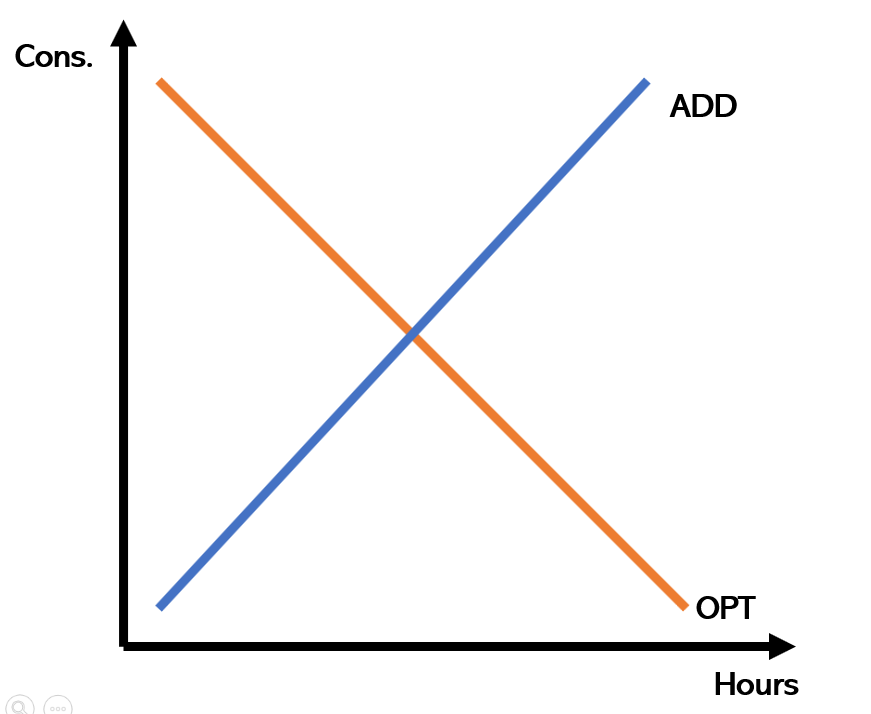
\includegraphics[scale=0.40]{images/RBC1-graph.PNG}
\end{center} 

\section{Dynamics and results}

\subsection{Shocks to $G$}

\subsubsection{Permanent positive shock to $G$}

The effects of a positive permanent shock to $G$ are all related to the downward shift of the ADD curve:
\begin{center}
 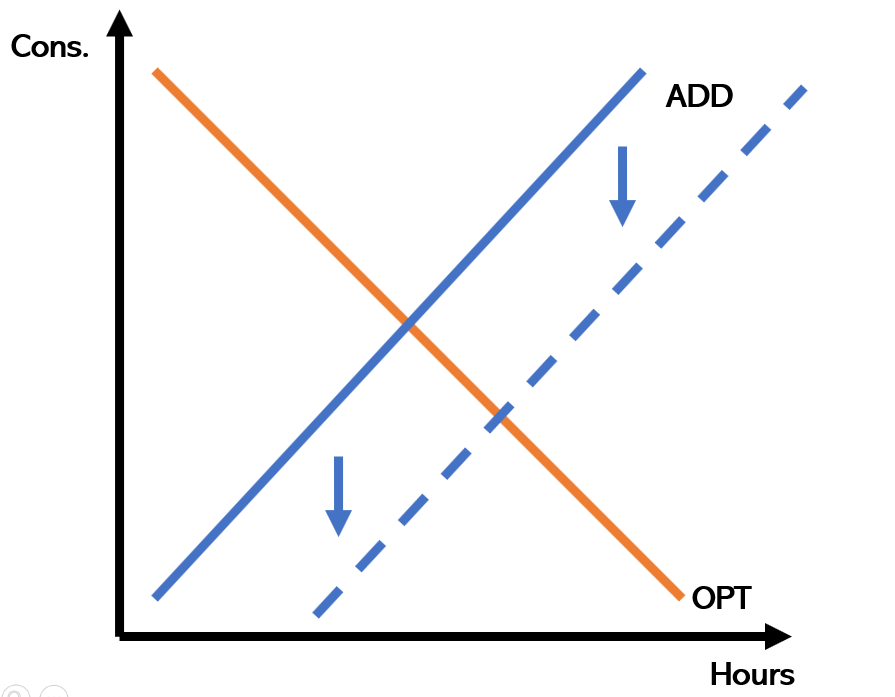
\includegraphics[scale=0.40]{images/RBC1-gshock.PNG}
\end{center}

This downward shift comes from the fact that setting higher taxes (increasing $G$) force people to consume less for the same amount of hours worked. However, since it is a lump-sum tax (no distortion), it does not affect the optimal share of consumption and labor directly.

From the graph, it is straightforward to see that:\begin{itemize}
\item[$C\downarrow$:] The shift of the ADD curve implies a drop in consumption.
\item[$H\uparrow$:] Hours worked also increase due to the shift of ADD.
\item[$W\downarrow$:] Since hours worked increase and capital is fixed, labor productivity is decreasing ($F_{HH}'' < 0$). In a fully competitive market, this means that wages go down.
\item[$Y\uparrow$:] Since hours worked increase and capital is fixed, output is increasing ($F_H' > 0$).
\item[$X\uparrow$:] A higher level of labor increases the marginal productivity of capital, hence increasing the return on the capital and dividends.
\item[$r\sim$:] A permanent change in $G$ will not affect the relative path of consumption. That means that the ratio $C_t/C_{t+1}$ will not change, hence no effect on interest rates.
\end{itemize}

\subsubsection{Temporary positive shock to $G$}

The effect on impact of the shock will be the same as the permanent shock for all variables except interest rates. As time goes by, all variables go back to their previous steady-state growth.

The difference in the interest rates variation comes from the perturbation of the consumption path. In fact, since consumption goes down on impact and comes back to its steady-state, we know that until the new equilibrium, consumption at $t+1$ will be higher than at $t$. This fact implies that a PIH consumer will want to smooth consumption by using future consumption today (i.e. borrowing). However, there is no vehicle to do so in this economy, the interest rate has to go up so that consumers do not want to borrow. We have that $r\uparrow$ following a positive temporary shock to $G$.

\subsection{Shocks to $Z$}

\subsubsection{Permanent shock to $Z$}

A positive shock to $Z$ will have two effects on the economy. First, it shifts ADD up as $C_t = Z_t F(\bar K, H_t) - G_t$. Second, it shifts OPT up as $C_t = \left(\frac{Z_t F_H'(\bar K, H_t)}{V'(\bar H - H_t)}\right)^{1/\sigma}$. The issue is that with two shifts in the same direction, we know that consumption will go up, but the effect on hours worked is unclear. Before exploring how we can make sense of this question, let's look at the graph and at the effects that are known:\begin{center}
 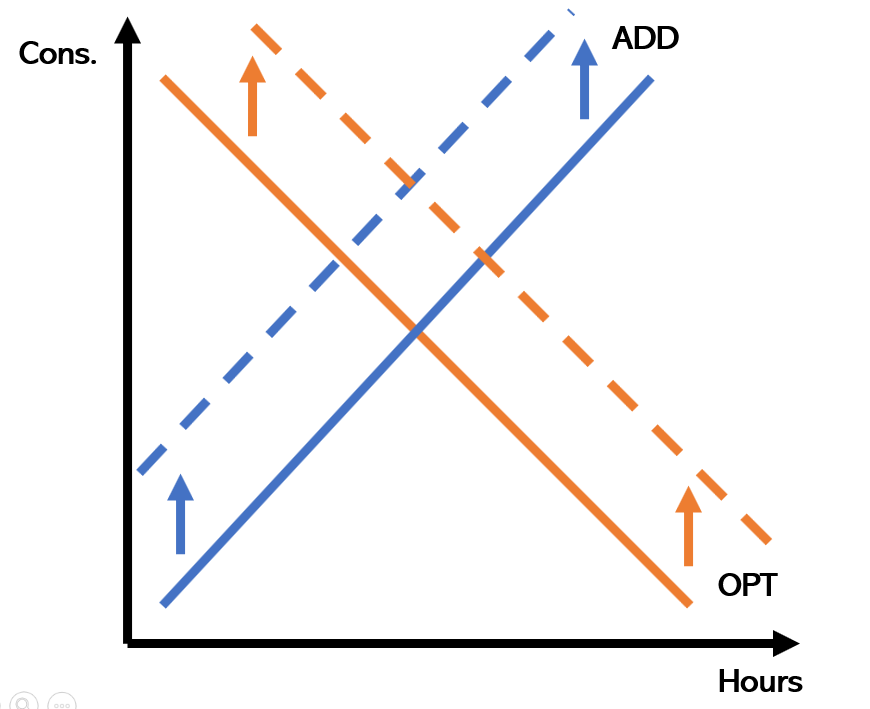
\includegraphics[scale=0.40]{images/RBC1-zshock.PNG}
\end{center}

\begin{itemize}
\item[$C\uparrow$:] Both curves movements imply an increase of consumption for the same leisure: hence, consumption goes up.
\item[$L$?:] The effects on the labor/leisure decision is indeterminate.
\item[$W\uparrow$:] Whatever the movement in hours worked, wages will increase following a left shift of labor supply and a right shift of labor demand.
\item[$Y\uparrow$:] Even without information on the effect on hours, we can safely assume that output will go up, since productivity icreases and the level of hours cannot be overly negative nor positive.
\item[$X\uparrow$:] Again, the fact that the effect on $H$ is not straightforward does not overpower the increase in productivity, leaving $X$ with a positive effect.
\item[$r\sim$:] A permanent change in $Z$ will not affect the relative path of consumption. That means that the ratio $C_t/C_{t+1}$ will not change, hence no effect on interest rates.
\end{itemize}

Now, in order to try and guess what actually happens to hours worked, consider writing both curves as functions of hours worked: $$\text{ADD: } \frac{C_t + G_t}{Z_t} = F(\bar K, H_t) \quad \text{ OPT: } \frac{C_t^\sigma}{Z_t} = G(H_t) $$ where $F$ is the production function (an increasing function in $H$, and $G$ is the ratio of wage to disutility in labor, a decreasing function in hours worked. If you divide both equations, you can study how the two effects work; for example, dividing OPT by ADD, you get approximately (without the government expenditures): $$C_t^{\sigma - 1} = \frac{G(H_t)}{F(\bar K, H_t)} $$ If $\sigma = 1$, meaning in the case of log utility, $C_t^{\sigma - 1} = 1$: both effects are equal, hours worked do not vary. If $\sigma < 1$, then an increase in $C_t$ will decrease the LHS, implying a decrease in the RHS: hours worked have to increase. In the opposite case, if $\sigma > 1$, then an increase in $C_t$ will increase the LHS, implying an increase in the RHS: hours worked have to decrease.

\subsubsection{Temporary shock to $Z$}

As studied in the government expenditures case, the effect on impact of a temporary shock will be the same as the permanent shock for all variables, except interest rates. However, here the consumption path will change in the opposite direction: consumption goes up first, then goes down, meaning consumption today will be higher than tomorrow until the new equilibrium. This means that consumers will want to save (i.e. buy consumption bonds); but as we now know, these bonds cannot be exchanged, therefore the interest rate has to decrease in order to make them less attractive. We have $r\downarrow$.

\section{Interpretation of the model}

\subsubsection{Summary of the results}

The summary of the model and its effects is in the table below:



We get that in response to shocks on $G$, consumption and wages go down, while output and hours worked react in the opposite direction. This means that they are countercyclical following a $G$ shock: this is not what we want to see from our model in terms of replication of actual observations.

Following a $Z$ shock however, all our variables seem to comove as we want them to, except for hours worked, which can go both ways.

These results are not quite satisfying since they do not show the actual data. This leads us to believe that the simple RBC model described here is (1) better for interpretation of the technology shocks, (2) lacking some key ingredients to make it more accurate. Moreover, one could argue that these effects are unconditional responses (the effect is alone, not affected by anything else). Impulse responses estimation would give a better result to show these conditional correlations. But in order to estimate an IRF, you need to identify the shocks hitting the economy, a hard task.

\subsubsection{Comovement of $C$ and $L$: the Barro-King problem}

We have seen two types of real shocks under the simplest RBC model: $G$ shocks and $Z$ shocks. The issue emphasized by Barro and King (1984) revolves around the fact that in the data, $H$ and $C$ seem to comove always. As we've seen, it is not the case following a shock on $G$ and can be also missed by a shock on $Z$. What can we do about it? We need to challenge the optimality conditions (OPT) such that they do move together.

\subsubsection{Technology shocks and labor supply}

We saw that technology shocks are close to reproducing the effects we see in the economy. But even if we consider only technology shocks, this simple RBC model is not as satisfying as we would want it to be. Indeed, hours worked are subject to both wealth and substitution effects, leaving it hardly variable following a $Z$ shock: the volatility of hours worked is not even close to output volatility. This issue calls for an amplification of labor supply shocks, meaning a very procyclical wage.

\section{Appendix}

\subsection{Fixed labor and capital: partial equilibrium RBC}

Suppose for the sake of it that labor is also supplied inelastically (as capital) like we had in the growth models of the first semester. What would the previously studied shocks deliver in terms of dynamics? Before trying to solve the model, note that supplying labor inelastically is the same as having a fixed amount of hours worked and of leisure, thereby fixing the marginal utility of leisure at $V'(\bar L)$ as well as the production function and its derivative (when you don't account for productivity).

\subsubsection{Productivity shock}



\subsection{Capital shock}



\subsection{News shocks}

A news shock is defined as a particular shock ($G$, $Z$ or anything else) that is expected to happen in the future. The dynamics following that type of shocks are different since consumers have time to take action before the shock. Indeed, since households are always looking to smooth consumption, any shock that has a future effect on $C$ will cause a current change on behavior. However, recall that this model does not include capital stock, nor consumption bonds in equilibrium. Hence, it is not possible for households to prepare for an event before it occurs. In order to wrap up our minds around this idea, let's use the example of a news shock on technology $Z$: in one period, a permanent shock on $Z$ will occur.

We already know what happens following a $Z$ shock under certain parameters: an increase in consumption and in output. In general, we can characterize this shock as making households richer. A richer household will generally work less, so labor supply shifts left immediately (even if the shock happens in one period). In contrast, labor demand will not shift out right away since the productivity gains have not yet happened. The combination of those effects in the labor market will cause hours worked to decrease and wages to increase on impact. This causes output to fall (hours worked fall while capital stock and productivity remain fixed). Moreover, a household that knows it will be consuming more in the following periods will want to smooth out this increase even today. But in this model, households have no vehicles of savings to sell in order to finance consumption now, they cannot increase consumption right away and the interest rate has to rise to compensate.

\chapter{Advanced RBC models}

As we advance into more complicated models, we need to discuss the full RBC model. A full RBC model means that we will introduce variable capital stock (investment) to our model, but we will also solve the  model numerically and simulate our way through shock analysis.

\section{Model}

\subsection{Households}

\subsubsection{Assumptions}

We use the typical model of household behavior, in which we allow for capital ($K_t$) accumulation via investment.Hence the only change to the problem will be on the budget constraint.

We get our usual multi-period objective function: $$\max_{C_t, H_t, K_{t+1}, B_{t+1}} \Et{\sum_{s=0}^{\infty} \beta^s \left( u(C_{t+s}) + V(\bar H - H_{t+s})\right)} $$ in which we assume that $u(C_t) = \ln(C_t)$ for simplicity. 

The budget constraint now allows for purchasing either consumption bonds (zero in equilibrium) yielding a return of $r_t$ or capital stock with a return $R_t$ that depreciates at a rate $\delta$. The household gets his income from previous periods assets, labor income and profits, while he has to pay for his consumption and taxes. Therefore the full budget constraint is written as: $$C_t + B_{t+1} + K_{t+1} = r_{t}B_t + [R_t + (1 - \delta)]K_t + W_tH_t + \Pi_t - T_t $$

This budget constraint can also be summarized as the national accounts identity: $Y = C + I + G$ where $I$ represents investment in the capital stock.

\subsubsection{Solution}

The solution to this problem is fairly similar to what we have seen in the previous chapter. Four FOCs are important: $$\frac{1}{C_t} = \lambda_t $$ $$V'(\bar H - H_t) = \lambda_t W_t $$ $$ \lambda_{t} = \Et{\beta(R_{t+1} + (1-\delta))\lambda_{t+1}} $$ $$\lambda_t = \Et{\beta r_{t+1}\lambda_{t+1}} $$ The last two equations are two sides on the same intuition: a Euler equation for risk-free bonds and one for risky assets. We will use the risky asset one for the actual Euler equation while transforming the risk-free condition into an arbitrage condition: $$ \Et{\beta(R_{t+1} + (1-\delta))\frac{\lambda_{t+1}}{\lambda_{t}}} = \Et{\beta r_{t+1}\frac{\lambda_{t+1}}{\lambda_{t}}} $$ $$\Leftrightarrow R_{t+1} \approx r_{t+1} + \delta + \text{ Risk premium} $$ And the Euler equation is given by: $$1 = \Et{\beta(R_{t+1} + (1-\delta))\frac{C_{t}}{C_{t+1}}} $$

\subsection{Firms}

Now we turn to the firm which is a very simple model in this RBC. As before, the production function is a neoclassical production function in capital and labor, augmented by technology $Z_t$ such that: $Y_t = F(K_t, Z_tH_t)$.

The firm's problem is to choose its capital and labor inputs and its output as to maximize profits in the following manner: $$\max_{Y_t, K_t, H_t} Y_t - W_tH_t - R_tK_t \text{ s.t. } Y_t = F(K_t, Z_tH_t) $$ which can be solved by replacing the constraint in the objective function in order to express it only as factor inputs. We get the following two FOCs: $$F_K(K_t, Z_tH_t) = R_t $$ $$ Z_tF_L(K_t, Z_tH_T) = W_t $$

\subsection{Government shocks}

As in the previous model, we assume government action is an exogenous process $T_t = G_t$ where $G_t$ is the exogenous process subject to shocks, either permanent or temporary. Note that government expenditures are not part of any utility or profits, they are pure waste.

The shocks on $G$ can be written in their dynamic form: $$\tilde G_{t+1} = \rho^G\cdot \tilde G_{t} + \varepsilon_{t+1}^G \text{ where } \Et{\varepsilon_{t+1}^G} = 0 $$

\subsection{Technology shocks}

Technology is also assumed to be an exogenous process, following the process: $$\tilde Z_{t+1} = \rho^Z\cdot \tilde Z_{t} + \varepsilon_{t+1}^Z \text{ where } \Et{\varepsilon_{t+1}^Z} = 0 $$

\subsection{Summary}

Before going further into solving the model, this section provides a summary of all equation and a small explanation on the interaction between them.

\subsubsection{Household Optimization}

$$\frac{1}{C_t} = \lambda_t $$ 
$$V'(\bar H - H_t) = \lambda_t W_t $$
$$1 = \Et{\beta(R_{t+1} + (1-\delta))\frac{C_{t}}{C_{t+1}}} $$

\subsubsection{Firm Optimization}

$$F_K(K_t, Z_tH_t) = R_t $$ 
$$ Z_tF_L(K_t, Z_tH_T) = W_t $$

\subsubsection{Constraints}

$$ Y_t = C_t + I_t + G_t $$
$$ K_{t+1} = (1 - \delta)K_t + I_t $$
$$ Y_t = F(K_t, Z_tH_t) $$

\subsubsection{Exogenous Shocks}

$$\tilde G_{t+1} = \rho^G\cdot \tilde G_{t} + \varepsilon_{t+1}^G $$
$$\tilde Z_{t+1} = \rho^Z\cdot \tilde Z_{t} + \varepsilon_{t+1}^Z $$

This sums up to a system of 10 non-linear equations that need to hold at the same time. This model is not easy to solve, and with that level of complexity there hardly is an analytical solution. Note that on the contrary to the previous model, capital is not fixed so we cannot reduce the dimensionality of the problem: we are now in a general equilibrium setting where the three markets (goods, assets, labor) have to clear at the same time. Solving this model will make use of new techniques developed in the following sections.

\section{Solving the model}

\subsection{Log-linearization}

Log-linearizing a system of equation allows to approximate a complex system of non-linear equations as an easy system of linear equations defined in the neighborhood of the steady state.

\subsubsection{Taylor expansion method}

Suppose $Z = F(X)$ is the function we want to log-linearize around the steady-state values $Z^* = F(X^*)$.

First, you take the logarithm on both sides: $$\ln(Z) = \ln(F(X))$$ Then, you use the Taylor expansion of order one to the steady state value: \begin{align*}
\ln(Z^*) + \frac{\partial\ln(Z^*)}{\partial Z} (Z - Z^*) & \approx \ln(F(X^*)) + \frac{\partial\ln(F(X^*))}{\partial X} (X - X^*) \\
\frac{1}{Z^*} (Z - Z^*) & \approx \frac{1}{F(X^*)}F'(X^*) (X - X^*) \\
\tilde Z & \approx \varepsilon_X \tilde X
\end{align*} where $\tilde{X} = \Delta\% X$ for any variable $X$ and $\varepsilon_X$ is the elasticity of function $F(\cdot)$.

We clearly got a linear relation between $X$ and $Y$, however, an unknown term was added, namely the elasticity of function $F(\cdot)$. This new parameter will need to be defined by the economist in a process called calibration.

\subsubsection{Basu's own method}

This shortcut consists in taking logs and totally differentiating, starting from the steady-state values. Again, let's use the same function $Z = F(X)$:\begin{enumerate}
\item Start with the steady state values: $Z^* = F(X^*)$
\item Take the logarithm of the equation: $\ln(Z^*) = \ln(F(X^*))$
\item Totally differentiate: $\frac{1}{Z^*}\D Z^* \approx \frac{1}{F(X^*)}F'(X^*)\D X^* $
\item Using the fact that $\D x \approx x - x^* $ and $\tilde x = \frac{x - x^*}{x^*}$, find the log-linear formulation: $$\tilde Z_t = \frac{F'(X^*)}{F(X^*)}\cdot \frac{X - X^*}{X - X^*} \D X^* $$ $$\Leftrightarrow \tilde Z_t = F'(X^*)\frac{(X - X^*)}{F(X^*)}\cdot \tilde X_t $$ $$\Leftrightarrow \tilde Z_t = \varepsilon_X^* \cdot \tilde X_t $$
\end{enumerate} 

\subsubsection{Case 1: the Euler equation}

Taking logs is impossible in this context since the presence of an expectation operator forbids to use any non-linear operator. We will have to start with totally differentiating:\begin{align*}
\lambda_t & = \Et{\beta\lambda_{t+1}( R_{t+1} + (1-\delta))} \\ 
\D\lambda_t & \approx \Et{ \beta(R^* + (1-\delta))\D\lambda_{t+1} + \beta\lambda^*\D R_{t+1}} \\
\D\lambda_t\cdot\frac{\lambda^*}{\lambda^*} & \approx \Et{ \beta(R^* + (1-\delta))\D\lambda_{t+1}\cdot\frac{\lambda^*}{\lambda^*} + \beta\lambda^*\D R_{t+1}\cdot\frac{R^*}{R^*}} \\
\tilde \lambda_t\cdot \lambda^* & \approx \Et{ \beta(R^* + (1-\delta))\tilde \lambda_{t+1}\cdot\lambda^* + \beta\lambda^*\tilde R_{t+1}\cdot R^*} \\
\tilde \lambda_t & \approx \Et{ \beta(R^* + (1-\delta))\tilde \lambda_{t+1} + \beta R^*\cdot\tilde R_{t+1} }
\end{align*} We now have a linear equation in expectation. Using the fact that in the steady state, $R^* + (1-\delta) = r^* = 1/\beta$, we can simplify our last equation to get: $$\tilde\lambda_t  \approx \tilde\lambda_{t+1} + \beta R^*\cdot\tilde R_{t+1}$$

\subsubsection{Case 2: the Production function (CRS + PC)}

We start with the assumption that the production function is of the form: $Y_t = F(K_t, Z_tH_t)$. Additional assumptions include that the firm is under perfect competition and that $F(\cdot)$ follows CRS.

This time, let's start by taking logs and taking the total differential:\begin{align*}
\ln(Y_t)&= \ln(F(K_t, Z_tH_t)) \\ \Leftrightarrow \tilde{Y}_t &\approx \frac{F_1(K^*, Z^*H^*)}{F(K_t, Z_tH_t)}\D K_t + \frac{F_2(K^*, Z^*H^*)}{F(K_t, Z_tH_t)}\big(\D Z_t + \D H_t\big) \\ \Leftrightarrow \tilde{Y}_t &\approx \varepsilon_{K} \tilde K_t + \varepsilon_{WH}(\tilde Z_t + \tilde H_t) \\
\end{align*}and we can use the fact that CRS implies that the elasticity of input is equal to the input share to write: $$\tilde{Y}_t \approx \left(1 - \frac{WH}{Y}\right)^* \tilde K_t + \left(\frac{WH}{Y}\right)^*(\tilde Z_t + \tilde H_t)$$ where the parameter to calibrate will be the share of labor in the production.

\subsubsection{Case 3: Labor demand}

Now, let's try with labor demand:\begin{align*}
Z_t \cdot F_L(K_t, Z_tH_t) & = W_t \\
\ln(Z_t) + \ln(F_L(K_t, Z_tH_t)) & = \ln(W_t) \\
\tilde Z_t + \frac{F_{LK}(K^*, Z^* H^*)}{F_L(K^*, Z^*H^*)}\D K_t + \frac{F_{LL}(K^*, Z^* H^*)}{F_L(K^*, Z^*H^*)}(\D Z_t + \D H_t) & = \tilde W_t \\
\tilde Z_t + \frac{F_{LK}(K^*, Z^* H^*)\cdot K^*}{F_L(K^*, Z^*H^*)}\tilde K_t + \frac{F_{LL}(K^*, Z^* H^*)\cdot(Z^*H^*)}{F_L(K^*, Z^*H^*)}(\frac{\tilde Z_t}{H^*} + \frac{\tilde H_t}{Z^*}) & = \tilde W_t \\
\end{align*}

\subsection{Calibration}

As we have seen, some variables are present in the log-linearized system without having been defined by the the model's condition. Hence, we must find values for these parameters that imply a correct specification for the economy. There are two solutions for this issue: calibration and estimation.

Estimation might be a more rigorous technique as it requires to use actual data to find parameter values. However, following this path might lead to few irregularities. First, estimation is a lot more difficult than calibration in the sense that you have to find data, a good model, robust analysis, etc. Second, you might not be able to estimate all parameters, depending on the data. In fact, the Minnesota school started a tradition to use steady-state data (average shares, average interest rates, etc.). The problem with this restriction is that it rules out some curvature parameters that cannot be present in steady-state data. Trying to get around this issue can also be problematic. For example, using micro-data may seem to be a good solution but it is often the case that sets of data are too restricted to say anything about aggregate behavior. Moreover, some might argue that there can be great differences between microeconomic conclusions and their aggregation.

In the end, calibrating seems to be the easiest choice, even though it leads to many strong debates in the profession. For now, we will keep it as is and talk more in depth about it later. 

\subsection{System of log-linearized equations}

In the end of that process, you should end up with a series of log-linearized equations, with parameters to fit in. This system of equations will help you solve dynamic stochastic general equilibrium models using Matlab (Dynare) or anything else.

Let's transform all our model equations into their respective log-linearized forms.

\subsubsection{Optimal consumption path}

$$1/C_t = \lambda_t \Leftrightarrow - \tilde C_t = \tilde \lambda_t $$

\subsubsection{Labor supply}

\begin{align*}
V'(\bar H - H_t) & = \lambda_t W_t \\
\Leftrightarrow- \frac{V''(\bar H - H^*)}{V'(\bar H - H^*)}\D H_t & = \tilde\lambda_t + \tilde W_t \\
\Leftrightarrow- \frac{V''(\bar H - H^*)\cdot (\bar H - H^*)}{V'(\bar H - H^*)\cdot (\bar H - H^*)}\cdot\frac{H^*}{H^*} \D H_t & = \tilde\lambda_t + \tilde W_t \\
\Leftrightarrow\underbrace{-\frac{V''(\bar H - H^*)\cdot (\bar H - H^*)}{V'(\bar H - H^*)}}_{\text{Elasticity of leisure marginal utility}} \cdot \underbrace{\frac{H^*}{(\bar H - H^*)}}_{\text{Ratio of hours to leisure}}\cdot \tilde H_t & = \tilde\lambda_t + \tilde W_t \\
\Leftrightarrow\tilde H_t & = \varepsilon_{HW} \cdot (\tilde\lambda_t + \tilde W_t) \\
\end{align*} 

\subsubsection{Euler Equation}

(See 5.2.1, case 1):

$$\tilde\lambda_t  \approx \tilde\lambda_{t+1} + \beta R^*\cdot\Et{\tilde R_{t+1}}$$

\subsubsection{Capital demand}

\begin{align*}
F_K(K_t, Z_tH_t) & = R_t \\
\Leftrightarrow \frac{F_{11}^*}{F_1^*}\D K_t + \frac{ F_{12}^*\cdot H^*}{F_1^*}\D Z_t + \frac{F_{12}^*\cdot Z^* }{F_1^*}\D H_t & = \tilde R_t \\
\Leftrightarrow \frac{F_{11}^*\cdot K^*}{F_1^*}\tilde K_t + \frac{ F_{12}^* \cdot Z^*H^*}{F_1^*}\tilde Z_t + \frac{ F_{12}^*\cdot Z^*H^*}{F_1^*}\tilde H_t & = \tilde R_t \\
\Leftrightarrow \frac{F_{11}^*\cdot K^*}{F_1^*}\tilde K_t + \frac{ F_{12}^* \cdot Z^*H^*}{F_1^*}\cdot (\tilde Z_t + \tilde H_t) & = \tilde R_t \\
\end{align*}
And since, from Euler's theorem, $F_1$ is of homogeneous degree 0, we can write: $$F_{11}^*\cdot K^* + F_{12}^* \cdot Z^*H^* = 0 $$ $$\Leftrightarrow - F_{11}^*K^*  =  F_{12}^* \cdot Z^*H^* $$ which leads to the following simplification:
\begin{align*}
\Leftrightarrow \frac{F_{12}^* \cdot Z^*H^*}{F_1^*}(\tilde Z_t + \tilde H_t - \tilde K_t) & = \tilde R_t \\
\Leftrightarrow \frac{F_2^*Z^*H^*\cdot F_{12}^* F^*}{F^*\cdot F_1^*F_2^*}(\tilde Z_t + \tilde H_t - \tilde K_t) & = \tilde R_t\\
\Leftrightarrow s_{H}\cdot \frac{1}{\varepsilon_{KH}}(\tilde Z_t + \tilde H_t - \tilde K_t) & = \tilde R_t \\
\end{align*}

\subsubsection{Labor demand}

(See 5.2.1, case 3):
$$ \frac{s_{K}}{\varepsilon_{KH}}(\tilde K_t - \tilde Z_t - \tilde H_t) = \tilde W_t  $$

\subsubsection{Aggregate resource constraint}

\begin{align*}
Y_t & = C_t + I_t + G_t \\
\Leftrightarrow Y_t - Y^* & = C_t - C^* + I_t - I^* + G_t - G^* \\
\Leftrightarrow \frac{Y_t - Y^*}{Y^*} & = \frac{C_t - C^* + I_t - I^* + G_t - G^*}{Y^*} \\
\Leftrightarrow \tilde Y_t  & = \tilde C_t \cdot \frac{C^*}{Y^*} + \tilde I_t \cdot \frac{I^*}{Y^*} + \tilde G_t \cdot \frac{G^*}{Y^*} \\
\Leftrightarrow \tilde Y_t  & = \tilde C_t \cdot s_C + \tilde I_t \cdot (1 - s_C - s_G) + \tilde G_t \cdot s_G \\
\end{align*}

\subsubsection{Law of motion of capital}

The law of motion of capital states that: $$K_{t+1} = (1 - \delta)K_t + I_t$$ and in the steady state, $K^* = (1 - \delta)K^* + I^* \Leftrightarrow I^* = \delta K^* $. Hence,
\begin{align*}
K_{t+1} & = (1 - \delta)K_t + I_t \\
\Leftrightarrow K_{t+1} - K^* & = (1 - \delta) K_t - K^* + \delta K^* + I_t - I^* \\
\Leftrightarrow \tilde K_{t+1} & = (1 - \delta)\frac{(K_t - K^*)}{K^*} + \frac{I^*}{K^*} \tilde I_t \\
\Leftrightarrow \tilde K_{t+1} & = (1 - \delta)\tilde K_t + \delta \tilde I_t \\
\end{align*}


\subsubsection{Production function}

(See 5.2.1, case 2):
$$\tilde{Y}_t \approx \left(1 - \frac{WH}{Y}\right)^* \tilde K_t + \left(\frac{WH}{Y}\right)^*(\tilde Z_t + \tilde H_t)$$

\subsubsection{Shocks}

$$\tilde G_{t+1} = \rho^G\cdot \tilde G_{t} + \varepsilon_{t+1}^G $$
$$\tilde Z_{t+1} = \rho^Z\cdot \tilde Z_{t} + \varepsilon_{t+1}^Z $$

\section{Dynamics and results}

\subsection{Shocks to $Z$}

Assume a shock to technology (productivity) $Z_t$. At first, we are not going to say anything about the persistency of the shock but we will see that at some point we will have to.

From our system of log-linearized equations, a shock to technology has a \textbf{direct} effect on:\begin{itemize}
\item \textbf{Capital demand:} a higher productivity means that capital stock will yield a greater marginal return, hence an increase in its price (perfect competition assumption). $$ s_{H}\cdot \frac{1}{\varepsilon_{KH}}(\tilde Z_t \uparrow + \tilde H_t - \tilde K_t) = \tilde R_t \uparrow $$
\item \textbf{Labor demand:} in the same way, a higher productivity means that labor will yield a greater marginal return, hence an increase in its price (perfect competition assumption). $$ \tilde Z_t + \frac{s_{K}}{\varepsilon_{KH}}(\tilde K_t - \tilde Z_t - \tilde H_t) = \tilde W_t  $$ $$ (1 - \frac{s_{K}}{\varepsilon_{KH}}) \tilde Z_t\uparrow + \frac{s_{K}}{\varepsilon_{KH}}(\tilde K_t - \tilde H_t) = \tilde W_t \uparrow $$
\item \textbf{Production:} however, since the production function is not an optimal equation but rather a constraint, let's leave it for later.
\end{itemize}

These effects increase current and future interest rates and wages which will also affect households in their wealth. While it could any way, our parametrization assumes that consumption will go up on impact. This effect is the main driver for determining the rest of the variables later.$ C\uparrow $

\subsubsection{Equilibrium in the labor market}

Now we turn to the labor market. Since we know that following a productivity shock we have a positive wealth effect, we can assume that labor supply will shift to the left. We already know that labor demand will go to the right. These two effects together will have the combined effect of rising wages (certainly) but the effect on hours worked in uncertain. Again, we use our parametrization to determine the direction of the effect: hours worked increase. $W\uparrow \quad H\uparrow $

\subsubsection{Equilibrium in the capital market}

The capital market is fairly easy to analyse on impact. We know that capital demand increased and since capital supply is fixed on impact (it takes one period to create capital), the interest rate will have to increase. $ R\uparrow $

\subsubsection{Investment and Output}

Finally, we can determine what happens to output and investment. Regarding investment, we know that households see an increase of consumption right on impact, while if the shock is transitory, they will want to smooth out this increase in wealth over periods, by investing (saving). This means that investment will go up on impact. From the resource constraint, we should observe an increase in output. Moreover, hours worked increased as well as productivity and capital will increase progressively. It is therefore now clear what happens to output: output should go up! $I\uparrow \quad Y\uparrow $

\subsubsection{Impulse response functions}

Now that we know what happens on impact, we can try and evaluate what are the potential dynamic effects in order to draw impulse response functions.

Since investment is up, the economy will experience capital accumulation for some periods (the capital stock will increase). This dynamic is not going to last as with time, less and less smoothing is required and both investment and consumption will start declining. An increasing capital stock will cause labor productivity to continue to rise and hence will shift labor demand to the right, pushing wages up. This effect will be higher as consumption continues to grow in the beginning but will be slowly decreasing once consumption starts going down. The effect on hours is still ambiguous but our estimated IRFs show that hours worked will go down. From the capital market, since capital supply will start to catch up (to the right), interest rates will slowly go down.

\begin{center}
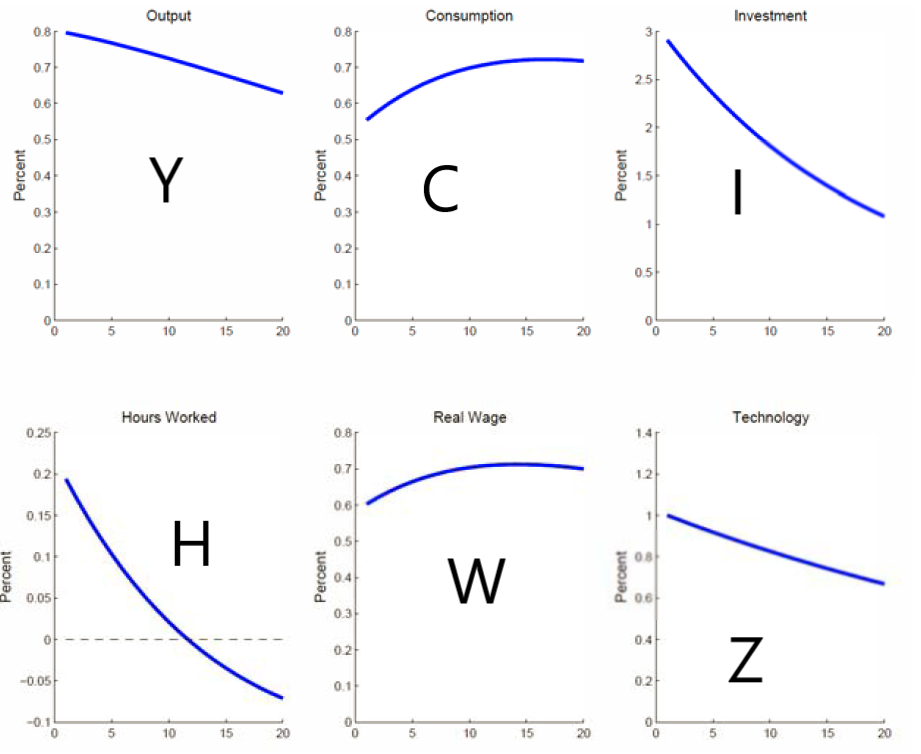
\includegraphics[scale=0.55]{images/RBC2-zshock.png} 
\end{center}

\subsection{Shocks to $G$}

Since government expenditures do not enter in neither household utility nor firm profits, a positive shock to $G$ is not going to produce great shocks to the optimal allocations between variables. Nevertheless, $G$ has a direct negative effect on the budget constraint, through taxes. This causes a negative wealth effect, forcing consumption to decrease on impact. Investment will decrease by even more to counteract the decrease of consumption. $C\downarrow \quad I\downarrow $

\subsubsection{Equilibrium in the labor market}

Consumers experience a loss of wealth, pushing them to work more for the same wages (to catch up for the loss), hence labor supply shifts to the right: hours worked increase and wages decrease. Labor demand is not affected on impact since $G$ has no effect on the firm and even though investment has gone down, it takes one period for capital to adjust and decrease. $H\uparrow\quad W\downarrow$

\subsubsection{Equilibrium in the capital market}

Nothing has changed in this market since neither capital supply (fixed on impact) nor capital demand (firm optimization) have changed on impact. $R\sim \quad K \sim$

\subsubsection{Output}

We have seen that both consumption and output will fall following a positive fiscal shock. This means that the effect on output we can observe from the resource constraint is unclear ($C, Y$ go down, $G$ goes up). However, we can see from employment that as hours worked go up, it should be the case that output goes up. $Y\uparrow$

\subsubsection{Impulse Response Functions}

Following the decrease of investment and consumption, and as the budget constraint progressively becomes less tight, we will see upward movements of both variables back to the steady state. Meanwhile, the fall in investment consumes some of the capital stock accumulated leaving $K$ to fall as well. A decrease in capital stock has a negative effect on labor productivity and a positive effect on capital productivity. Hence, labor demand will shift out, and with labor supply shifting back, we will see wages going back up and hours going down. Capital productivity going up means a shift of capital demand to the right while capital supply goes to the left: we can expect an increase in the interest rate.

\begin{center}
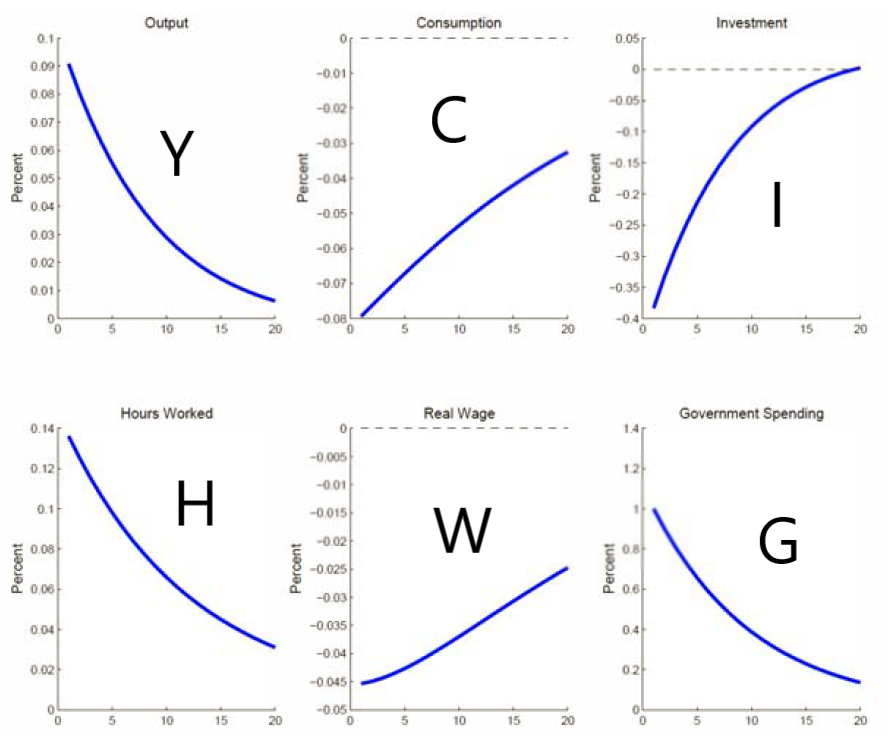
\includegraphics[scale=0.55]{images/RBC2-gshock.png} 
\end{center}

\section{Interpreting the results}

In order to assess the efficiency of the RBC model, one must define criterias against which it is possible judge the output of the model. Cooley and Prescott (1995) are among the earliest to do this and they choose to match relative volatilities of key moments.

For instance, take a one-time unique technology shock. The benchmark RBC model will predict:\begin{itemize}
\item $\sigma_I > \sigma_Y > \sigma_C$ : that is, investment is the most volatile component while consumption is relatively smooth in comparison to output.
\item Variables $Y, I, C$ and $H$ will commove following a shock.
\end{itemize}

However, the model has some inconsistencies with the data. In particular, the model does not generate enough  volatility  of  interest rates.  Further, it generates wages and real interest rates that are far too procyclical relative to the data.  In the data, wages are very modestly procyclical and real interest rates are acyclical or countercyclical, depending on how you measure them. Moreover, the variations of $C$ and $H$ are too smooth compared to actual observations. As a result, labor productivity will be too much correlated with output (since $H$ doesn't change), also something that is not observed. It also seems that $r$, the interest rate is too strongly procyclical. Finally, at a deeper level, people have criticized RBC models because they don’t seem particularly
realistic.  To generate fluctuations that resemble those in the US, one needs large, high frequency
variation in $Z_t$. The issue here is that a technology shock must be present to move the model, but it seems highly unprobable to have a negative shock to technology to model recessions.

After thorough analysis, it seems that the RBC model makes a lot of mistakes when compared to actual observations. The first counterargument to this apparent issue is to ask if we can really compare the shocks fed into the RBC model to shocks happening in real life. In fact, RBC shocks are unique and unconditional, meaning nothing else happens at the same time. We have studied that some shocks (in particular shocks on $G$) can affect consumption the other way: could it be that real life shocks are affected by different contradictory shocks at the same time? Probably. Hence, we should theoretically feed the model with the same mix of shocks that happen in the data: this is very difficult to do.

Critics of the real business cycle model are uncomfortable with the facts that it is (a)
driven by technology “shocks” and that (b) these shocks must be large and sometimes negative.
Hence, much of business cycle research since the 1980s has been involved in modifying the basic
model  to  (a)  allow  other  shocks  to  “matter”  in  a  way  that  they  can’t  in  the  basic  model (e.g. monetary policy) and (b) generating better and more realistic mechanisms for the model to take “small” shocks (as opposed to large) and produce relatively large business cycles.

\section{Appendix}

\subsection{Capital Shocks}

\subsection{Patience shocks}

In the models we described since the beginning, we have used the parameter $\beta\equiv\frac{1}{1+\rho}$ to represent the “patience" of households. In particular, a high $\beta$ means that households value future utility very much (i.e. they are patient) while a low $\beta$ means the exact opposite. We will see later that patience can be very important to model as it is a defining characteristic of the quantity of goods a households wants now instead of later. That's why we look at this type of shocks in the case of our second RBC model (with capital).

Let's assume a negative shock to $\beta$, meaning households would rather consume more now than they used to. From the Euler equation, we can see that this has a clear negative effect on the current Lagrangian multiplier $\lambda_t$ meaning that this is equivalent to a positive wealth effect: people feel richer. This means that:\begin{itemize}
\item Current consumption goes up.
\item Labor supply shifts left: hours worked decrease and wages increase.
\item Output decreases as hours worked decreases.
\item Consumption goes up while output goes down: investment must go down.
\end{itemize}

\subsection{Laziness shocks}

In this particular case, suppose that marginal utility derived from leisure increases. In order to see that in an easier manner than with the general $V(\bar H - H_t)$, let's assume that utility from leisure takes the following form: $$V(\bar H - H_t)\equiv \theta\ln(\bar H - H_t) $$ Then a shock to laziness could be modeled as a shock to the parameter $\theta$.

When this happens, you could compare it to increased laziness of households and hence it will cause a shift to the left to the labor supply, without affecting labor demand: wages go up and hours worked go down. We can also argue from the combination of all FOCs that consumption will decrease as well. Moreover, if hours worked decrease, then output decreases as well since productivity and capital stock didn't change. In general, this shock functions as a negative wealth effect, which will force households to decrease investment in order to smooth consumption. Finally, since the capital stock slowly decreases after impact, the interest rate will increase.

\subsection{News shocks}

As we have seen in the previous chapter, news shocks work like wealth shocks in the sense that households expect what is going to happen in the future. Let's use the example of a positive news shock.

Households feel richer and hence will:\begin{itemize}
\item Increase current consumption (because of smoothing)
\item Reduce their labor supply (they don't need to work so much anymore)
\item Reduce investment (again because of smoothing)
\end{itemize}
This will additionally cause output to go down, wages to go up, interest rates to go up progressively.

\subsection{Uncertainty shocks}



\chapter{Non-Walrasian RBC models}

\section{Externalities in production}

This chapter will uncover some of the effects implied by extreme marginal products in production. The rationale behind this theory is to try and get out of the result that only a shock in $Z$ will make $Y, C, I$ and $H$ comove. We could also use the rationale that facts are not matched yet and we would want to find other theories that could potentially lead to better matching models. In order to do this, we'll introduce increasing marginal products via Marshallian externalities: the classical assumption that when firms produce more, other firms get more productive. 

\subsection{Model}

\subsubsection{Firms} 

As we will see, the main difference between this model and the previous one is how firms are modeled. In particular, instead of having one representative firm, we will have a continuum of firms, indexed by $i$ where $i\in[0,1]$. Each firm will have the same production technology (function) but will produce a different output, denoted $Y_{it}$ (output produced by firm $i$ at time $t$). The production function is given by: $$ Y_{it} = A_t\cdot K_{it}^\alpha (Z_tH_{it})^{1-\alpha} $$ The main difference between this production function and the one in previous models is that $A_t$ is a new variable, called the externality. As you can see, $A_t$ is not so different than $Z_t$ in the firm's view as it is an exogenous, time-varying input. 

Nevertheless, $A_t$ will play a different role in the whole economy as it is in fact an endogenous variable for the economy as whole. In fact, we define $A_t$ as an increasing function of aggregate output $Y_t$: by producing more firms get more productive, but they do not internalize this process. Formally, $$A_t = Y_t^{1 - \frac{1}{\gamma}} = \left[\int_{0}^1 Y_{it}\D i\right]^{1 - \frac{1}{\gamma}} $$ The aggregate stock of capital $K_t$ and labor $H_t$ are defined in the same way as aggregate output. From that aggregation, the whole economy's production function will be slightly modified: \begin{align*}
Y_t = \int_{0}^{1} Y_{it}\D i \Leftrightarrow Y_t = \int_{0}^{1}A_tK_{it}^\alpha (Z_tH_{it})^{1-\alpha}\D i \Leftrightarrow & Y_t = \int_{0}^{1}Y_t^{1-\frac{1}{\gamma}}K_{it}^\alpha (Z_tH_{it})^{1-\alpha}\D i\\ \Leftrightarrow & Y_t = Y_t^{1-\frac{1}{\gamma}}\int_{0}^{1}K_{it}^\alpha (Z_tH_{it})^{1-\alpha}\D i \\ \Leftrightarrow & Y_t^{\frac{1}{\gamma}} = \int_{0}^{1}K_{it}^\alpha (Z_tH_{it})^{1-\alpha}\D i \\ \Leftrightarrow & Y_t = \left[ \int_{0}^{1}K_{it}^\alpha (Z_tH_{it})^{1-\alpha}\D i\right]^{\gamma} \\ \Leftrightarrow & Y_t = \left[ K_{t}^\alpha (Z_tH_{t})^{1-\alpha}\right]^{\gamma} 
\end{align*}

The individual firm's problem is now: $$\max_{K_{it}, H_{it}} A_tK_{it}^\alpha (Z_tH_{it})^{1-\alpha} - W_tH_{it} - R_tK_{it} $$ yielding the following two FOCs (or input factor demands): $$\alpha A_t K_{it}^{\alpha - 1} (Z_tH_{it})^{1-\alpha} = R_t $$ $$\text{and }(1 - \alpha) A_t K_{it}^{\alpha} Z_t^{1-\alpha} H_{it}^{-\alpha} = W_t $$ We know that $A_t = \left(\left[ K_{t}^\alpha (Z_tH_{t})^{1-\alpha}\right]^{\gamma}\right)^{1 - \frac{1}{\gamma}} = K_t^{\alpha(\gamma - 1)}(Z_tH_{t})^{(1-\alpha)(\gamma - 1)}$. Moreover, in equilibrium, it must be that all firms have the same level of inputs (since the prices are the same for all firms and they are price-takers in input markets). This means that $K_{it} = K_{jt}$ for any $i, j$. Therefore, $$K_t = \int_0^1 K_{it}\D i = K_{it} \int_0^1 1\D i = K_{it} $$ and the same applies for labor, $H_t = H_{it}$.

Consequently, we have a new formula for labor demand: \begin{align*} 
W_t & =  (1 - \alpha)K_t^{\alpha(\gamma - 1)}(Z_tH_{t})^{(1-\alpha)(\gamma - 1)}  K_{t}^{\alpha} Z_t^{1-\alpha} H_{t}^{-\alpha} \\
& = (1 - \alpha) K_t^{\alpha\gamma} Z_t^{(1-\alpha)\gamma} H_{t}^{(1-\alpha)\gamma - 1}
\end{align*}
which in turn gives a new log-linearized equation: $$\tilde{W}_t = \alpha\gamma \tilde K_t +\gamma(1-\alpha) \tilde Z_t + [(1-\alpha)\gamma - 1] \tilde H_t $$ And a new formula for capital demand:\begin{align*} 
R_t & =  \alpha K_t^{\alpha(\gamma - 1)}(Z_tH_{t})^{(1-\alpha)(\gamma - 1)}  K_{t}^{\alpha - 1} (Z_tH_{t})^{1-\alpha} \\
& = \alpha K_t^{\alpha\gamma - 1} (Z_tH_{t})^{(1-\alpha)\gamma}
\end{align*}
which in turn gives a new log-linearized equation: $$\tilde{R}_t = (\alpha\gamma - 1)\tilde K_t +(1-\alpha)\gamma [\tilde Z_t +  \tilde H_t] $$

These two input factor demands may not seem different than the usual ones, however the externality parameter $\gamma$ holds an important change: their slopes are now linked to $\gamma$. For example, when $\gamma$ increases (externalities increase) the labor demand curve gets flatter and flatter, until it reaches positive territory: labor demand is sloping up! A positive slope of labor demand would give new interpretations for shocks, but it could also lead to non-convergent steady-states, ultimately ruining our model. We must first make sure that there is in fact a steady-state around which we log-linearize. The requirement for an existing steady-state is that $\gamma\alpha < 1 \Leftrightarrow \gamma < 1/\alpha \Leftrightarrow \gamma<3$. For labor demand to slope up we need $(1-\alpha)\gamma - 1 > 0 \Leftrightarrow \frac{1}{1-\alpha} < \gamma \Leftrightarrow \gamma > 3/2$. We'll therefore look at effects under values of $\gamma$ lying between $[1.5 , 3)$.

Finally, let's log-linearize the aggregate production function: $$ Y_t = \left[ K_{t}^\alpha (Z_tH_{t})^{1-\alpha}\right]^{\gamma} $$ $$\Leftrightarrow \tilde Y_t = \gamma\alpha \tilde K_t + \gamma(1-\alpha)(\tilde Z_t + \tilde H_t) $$ 

\subsubsection{Rest of the model}

In essence, the rest of the model is our typical RBC model so we are not going to detail the computations here. However, a summary of the  system of log-linearized equations is provided below:

\textbf{Optimal consumption path:} $$ - \tilde C_t = \tilde \lambda_t $$

\textbf{Labor supply:}$$ \tilde H_t = \varepsilon_{HW} \cdot (\tilde\lambda_t + \tilde W_t) $$

\textbf{Euler Equation:}$$\tilde\lambda_t  \approx \tilde\lambda_{t+1} + \beta R^*\cdot\Et{\tilde R_{t+1}}$$

\textbf{Aggregate resource constraint:}$$ \tilde Y_t  = \tilde C_t \cdot s_C + \tilde I_t \cdot (1 - s_C - s_G) + \tilde G_t \cdot s_G $$

\textbf{Law of motion of capital:}$$ \tilde K_{t+1} = (1 - \delta)\tilde K_t + \delta \tilde I_t $$

\textbf{Shocks:}

$$\tilde G_{t+1} = \rho^G\cdot \tilde G_{t} + \varepsilon_{t+1}^G $$
$$\tilde Z_{t+1} = \rho^Z\cdot \tilde Z_{t} + \varepsilon_{t+1}^Z $$

\subsection{Results}

For the results of this model, keep in mind that the reasoning is approximately the same as in classical RBC models, only with an upward-sloping demand for labor. This will help us to identify easily the quantitative differences that are caused by externalities. To do that, we consider three models: the classical RBC (no externalities), a moderate level of externalities and high externalities.

\subsubsection{Shocks to $G$}

A shock to $G$ is essentially a negative wealth effect, pushing labor supply down. In the classical RBC model, this caused an increase in hours worked and a decrease in wages. With externalities however, labor demand is sloping up, which translates into higher wages in addition to higher hours worked. This could even mean that consumption could rise. In fact, in the RBC model, income does not change that much since wages and hours move in different direction and overall taxes increase. In the models with externalities, the common increase in both hours and wages could potentially offset taxes increase. As we can see from the graphs below, a moderate level of externalities might not be enough, while a high level would do the work.\begin{center}
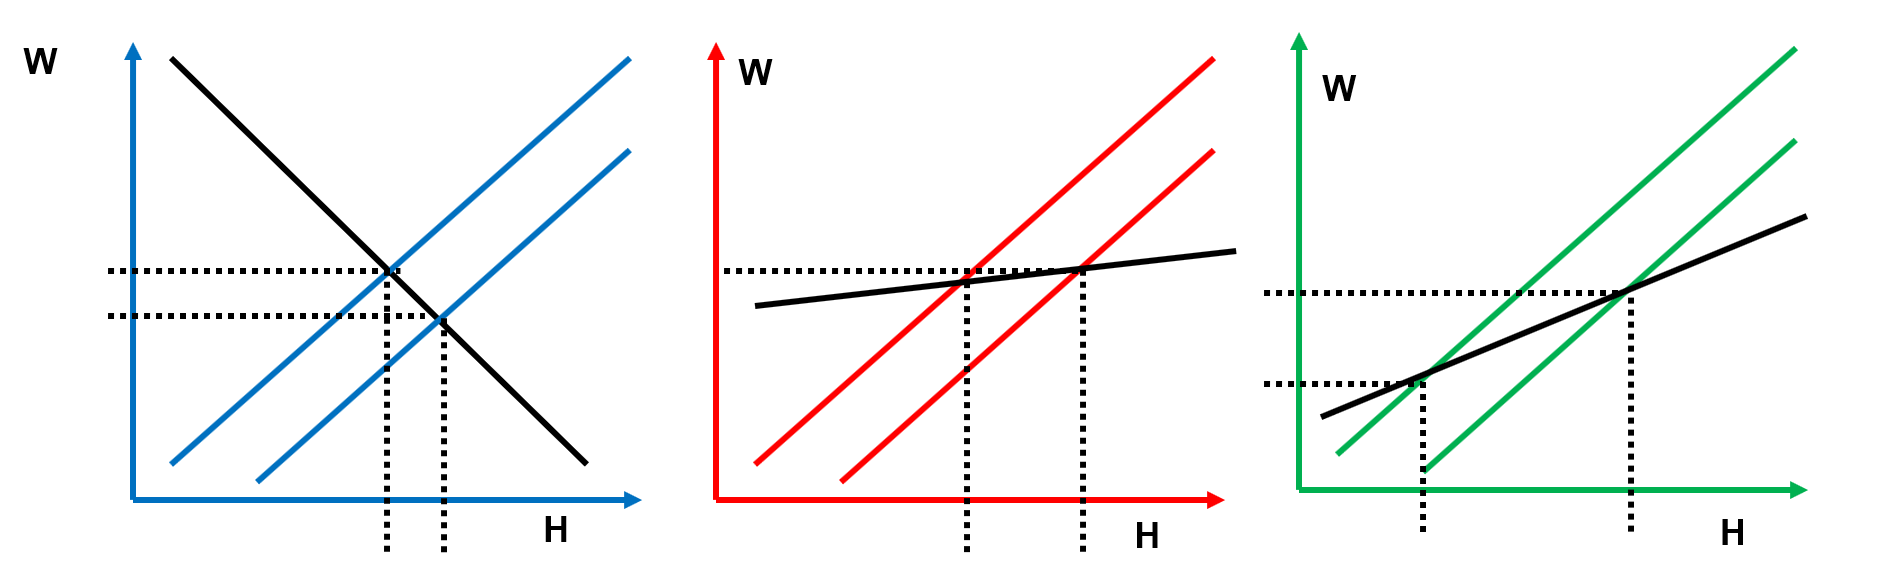
\includegraphics[scale=0.275]{images/RBC3-gshock0.PNG} 
\end{center}

We also know that higher number of hours will mean higher output, an effect that will be emphasized as externalities are more and more important, and consumption suffers less and less from taxes. The direction of consumption will also change what happens with investment. It will be going down when consumption goes down but up in the cases with externalities. The direction of consumption is the same in all cases and therefore interest rate will go up on impact and go down. $$ C\uparrow ; H\uparrow ; W\uparrow ; Y \uparrow ; I\uparrow $$ You can see the IRFs of the aforementioned shock below. Note that the blue line shows the RBC case, while green and red lines show the effects under externalities. \begin{center}
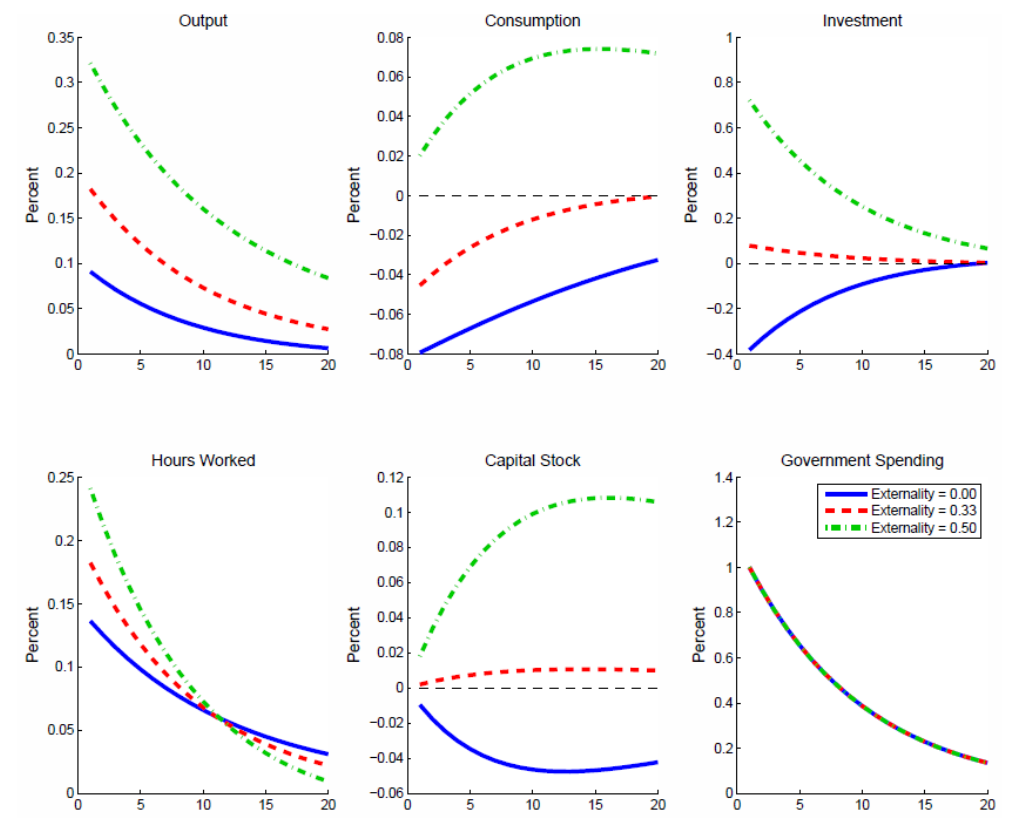
\includegraphics[scale=0.4]{images/RBC3-gshock1.PNG} 
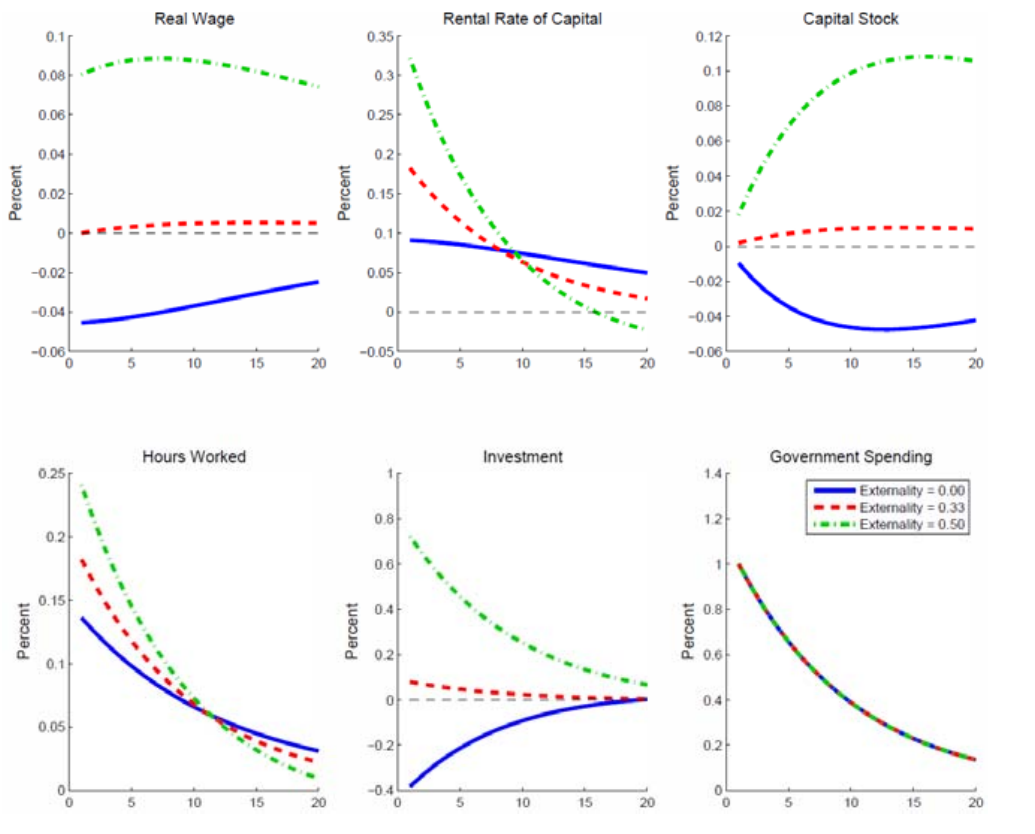
\includegraphics[scale=0.4]{images/RBC3-gshock2.PNG} 
\end{center}

\subsubsection{Shocks to $Z$}

A shock to $Z$ will have: (1) a positive wealth effect for households and (2) a positive effect on input marginal returns for firms.

Therefore, in the labor market, labor supply shifts to the left while labor demand shifts to the right. Since labor demand is now sloping up, this creates increasing wages and hours worked (less ambiguous than in classical RBC models). The increase of hours worked also means an increase in output. 

In the capital market, the increase in productivity implies higher capital demand, thus a higher interest rate. Investment goes up as households smooth consumption, meaning that capital stock increases progressively, bringing back the interest rate to its steady-state.$$ C\uparrow ; H\uparrow ; W\uparrow ; Y \uparrow ; I\uparrow $$ You can see the IRFs of the aforementioned shock below. Note that the blue line shows the RBC case, while green and red lines show the effects under externalities. \begin{center}
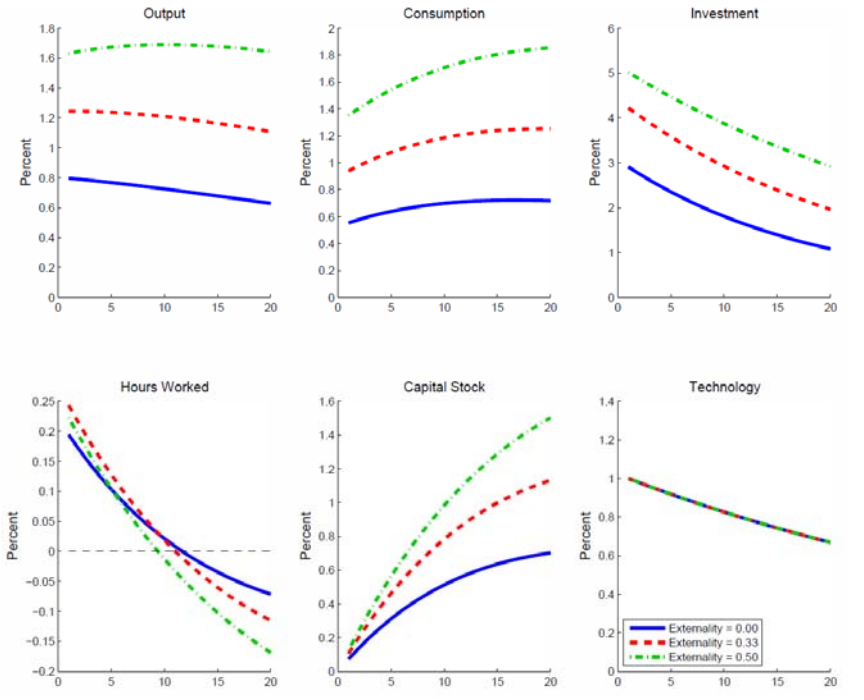
\includegraphics[scale=0.4]{images/RBC3-zshock1.PNG} 
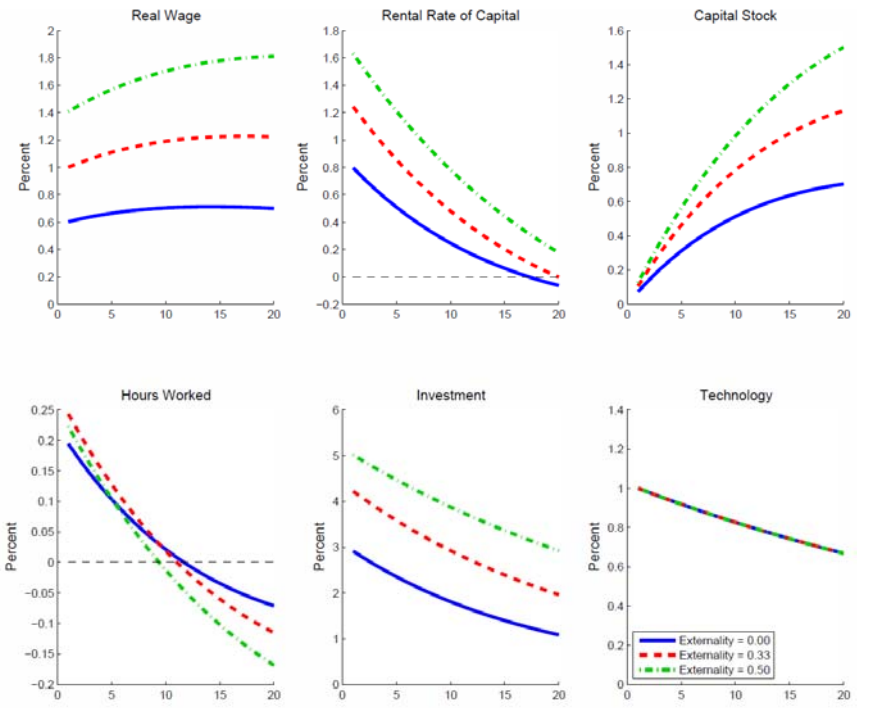
\includegraphics[scale=0.4]{images/RBC3-zshock2.PNG} 
\end{center}

\subsection{Interpretation}

The main results to draw from this new model is how externalities allow for commovement oh $C$ and $H$, even when the shocks are not technologically driven! The key to that commovement relies on endogenous shifts in labor demand at the firm level. This is very interesting to both reasons we delved into the model in the first place. However, there seems to be very little evidence that in fact those kind of externalities happen in the data. Therefore we might look for other ways to implement the same type of endogeneity of firm labor demand in a new manner.

\section{Imperfect Competition: the Rotemberg-Woodford model}

This section's topic is imperfect competition and its implications for the typical DSGE models. Imperfect competition is important since:\begin{itemize}
\item It allows for more realism (describes actual situations where firms indeed hold some market power).
\item It allows to study situations in which at the firm level there are increasing returns (see previous chapter).
\item It allows non-technological shocks to have desired effects on the model (think demand shocks or even sunspot shocks).
\item It has different predictions as to the effects of technological shocks.
\end{itemize}

\subsection{Model}

\subsubsection{Demand for differentiated goods}

This model assumes a different kind of aggregation for products. We've seen in the previous that although firms produce different products, they all sold at the same price. This time we relax this assumption.

Let there be a continuum of differentiated commodities indexed by $i\in[0,1]$ such that a unique firm produces a unique good that other firms cannot match. Those goods are somewhat substitutable. The aggregate demand in the economy ($C, I$ and $G$) is for the composite good $Y$ where $$Y_t = \left[\int_0^1 y_{it}^{(\sigma -1)/\sigma}\D i\right]^{\sigma/(\sigma -1)}$$ In this equation, the new parameter $\sigma$ is the price-elasticity of demand. It is required to be strictly greater than 1.

All users of output solve: $$\min_{y_{it}}\int_0^1 p_{it}y_{it}\D i \text{ }\text{ s.t. } Y_t = \left[\int_0^1 y_{it}^{(\sigma -1)/\sigma}\D i\right]^{\sigma/(\sigma -1)} $$ This problem has the following FOC: $$p_{it} - \psi_ty_{it}^{-1/\sigma}\left[\int_0^1 y_{it}^{(\sigma -1)/\sigma}\D i\right]^{1/(\sigma -1)} = 0$$ $$\Leftrightarrow y_{it} = \left(\frac{p_{it}}{\psi_{t}}\right)^{-\sigma} \left[\int_0^1 y_{it}^{(\sigma -1)/\sigma}\D i\right]^{\sigma/(\sigma -1)} $$ $$ \Leftrightarrow y_{it} = \left(\frac{p_{it}}{\psi_{t}}\right)^{-\sigma} Y_t$$ And we can solve for $Y_t$ in:\begin{align*}
Y_t = \left[\int_0^1 \left(\frac{p_{it}}{\psi_{t}}\right)^{1-\sigma} Y_t^{(\sigma -1)/\sigma}\D i\right]^{\sigma/(\sigma -1)} & \Leftrightarrow Y_t = \left[\left(\frac{Y_t^{(\sigma -1)/\sigma}}{\psi_{t}^{1-\sigma}}\right) \int_0^1 p_{it}^{1-\sigma} \D i\right]^{\sigma/(\sigma - 1)} \\ & \Leftrightarrow Y_t = \left[\left(\frac{Y_t}{\psi_{t}^{1-\sigma}}\right) \int_0^1 p_{it}^{1-\sigma} \D i\right]^{\sigma/(\sigma - 1)} \\
& \Leftrightarrow \psi_{t}^{\frac{(\sigma - 1)\sigma}{(1-\sigma)}} = \left[\int_0^1 p_{it}^{1-\sigma} \D i\right]^{\sigma/(\sigma - 1)} \\
& \Leftrightarrow \psi_{t} = \left[\int_0^1 p_{it}^{1-\sigma} \D i\right]^{1/(1 - \sigma)} = P_t
\end{align*} Which gives our final demand that the producer faces: $$y_{it} = \left(\frac{p_{it}}{P_t}\right)^{-\sigma}Y_t $$

\subsubsection{Firms}

Let each firm be a monopoly for the good market that it produces. Then, the optimization problem of the firm is: $$\max_{p_{it},h_{it},k_{it}} p_{it}y_{it} - W_th_{it} - R_tk_{it} \text{ }\text{ s.t. } y_{it} = F(k_{it}, Z_th_{it}) - \Phi $$ where $h,k$ are firm-level inputs and $\Phi$ is a fixed cost. We can replace $y_{it}$ by the demand function derived earlier. This yields the following Lagrangian: $$\mathcal{L}\equiv p_{it}\left(\frac{p_{it}}{P_t}\right)^{-\sigma}Y_t - W_th_{it} - R_tk_{it} +\phi_{it}\left[F(k_{it}, Z_th_{it}) - \Phi - \left(\frac{p_{it}}{P_t}\right)^{-\sigma}Y_t\right] $$
the first-order conditions are:\begin{itemize}
\item Price: $$(1 - \sigma)\left(\frac{p_{it}}{P_t}\right)^{-\sigma}Y_t - \phi_{it}(-\sigma)\left(\frac{p_{it}^{-\sigma - 1}}{P_t^{-\sigma}}\right)Y_t = 0 $$ $$\Leftrightarrow (1-\sigma) = \phi_{it}(-\sigma)p_{it}^{-1} $$ $$ p_{it} = \phi_{it}\cdot\frac{\sigma}{\sigma - 1} $$
\item Labor: $$W_t = \phi_{it}Z_tF_2(k_{it}, Z_th_{it}) $$
\item Capital: $$R_t = \phi_{it}F_1(k_{it}, Z_th_{it}) $$
\end{itemize} 
You can observe that $\phi_{it}$, the Lagrangian multiplier of the production constraint, can be interpreted as the cost of producing one more unit of output at the equilibrium. In other words, it is the marginal cost of the firm at the optimal level. Now, because the price is a function of the marginal cost, we will define $\frac{\sigma}{\sigma - 1}$ as the markup, denoted $\mu$. We can hence simplify our system of FOCs into: $$\phi_{it} = \frac{1}{\mu} p_{it} $$ $$\mu W_t = p_{it}Z_tF_2(k_{it}, Z_th_{it}) $$ $$\mu R_t = p_{it}F_1(k_{it}, Z_th_{it}) $$ This formulation makes it clear that, since all firms are price-takers on the input markets, they must have the same input levels as well as the same price: this is a symmetric equilibrium. Therefore, as in the previous model: $$p_{it} = P_t; y_{it} = Y_t ; k_{it} = K_t ; h_{it} = H_t $$ We can therefore normalize the price level to 1 to get: $$\phi_t = \frac{1}{\mu} $$ $$W_t = \frac{1}{\mu} Z_tF_2(k_{it}, Z_th_{it}) $$ $$R_t = \frac{1}{\mu} F_1(k_{it}, Z_th_{it}) $$

\subsubsection{Log-linearizing the new equations}

In order to solve this new model, we need to log-linearize the four new equations we got.

This is a fairly easy task for the marginal cost and input factor demands as not much has changed. In fact, the marginal cost does not change at all, and since $\mu$ is fixed, the two input demands have not changed either. $$ \tilde W_t = \alpha [\tilde K_t - \tilde H_t] + (1-\alpha)\tilde Z_t $$ $$ \tilde R_t = (1-\alpha)[\tilde H_t + \tilde Z_t - \tilde K_t] $$

For the production function, we have that $Y_t + \Phi	= F(K_t, Z_tH_t) $, by taking logs and totally differentiating you get:\begin{align*}
Y_t + \Phi = F(K_t, Z_tH_t) \Leftrightarrow  \ln(Y_t + \Phi) & = \ln(F(K_t, Z_tH_t)) \\
\Leftrightarrow  \frac{1}{Y^* + \Phi}\D Y_t & = s_K \tilde{K}_t + (1 - s_K)(\tilde{Z}_t + \tilde{H}_t)\\
\Leftrightarrow  \frac{Y^*}{Y^* + \Phi}\tilde Y_t & = s_K \tilde{K}_t + (1 - s_K)(\tilde{Z}_t + \tilde{H}_t)
\end{align*} This form helps us see an interesting effect of fixed cost on production. Assume output grows by one dollar ($\tilde Y_t\uparrow$), growth of inputs has increased by $\frac{Y^*}{Y^* + \Phi}$ dollars, which is less than one. We get increasing returns to scale. We define $\gamma \equiv \frac{Y^*+ \Phi}{Y^*}$ in order to emphasize on the similarity with the previous model.

Because $\gamma$ represents returns to scale, we can also write it as: $$\gamma = \frac{\text{Average Cost}}{\text{Marginal Cost}} = \frac{\mathcal{C}(\cdot)/Y}{\mathcal{C}'(\cdot)} = \frac{P\cdot\mathcal{C}(\cdot)}{\mathcal{C}'(\cdot)\cdot PY} = \mu(1 - s_\pi) $$ where $\mu$ is the markup (as defined above) and $s_\pi$ represents the profit share in total revenues. In the steady-state, profits should be equal to 0, leaving us with the fact that $\gamma = \mu$ in the steady-state. We can therefore write: $$\tilde Y_t = \mu \alpha \tilde K_t + \mu (1 - \alpha)[\tilde Z_t + \tilde H_t] $$

\subsubsection{Rest of the model}

In essence, the rest of the model is our typical RBC model, but there is a single main difference: potential profits. Indeed, remember that the budget constraint of the representative household includes a profit term $X_t$ or $\Pi_t$. Usually, this term is zero always since firms are perfectly competitive but in this model, firms might make some profits out-of-equilibrium. Indeed, recall that increasing inputs will create more output than a one-to-one until we come back to the steady-state. This fact is important to keep in mind as it can introduce shocks to markups.

As before, we are not going to detail all the computations of the rest of log-linearizations here. However, a summary of the  system of log-linearized equations is provided below:

\textbf{Optimal consumption path:} $$ - \tilde C_t = \tilde \lambda_t $$

\textbf{Labor supply:}$$ \tilde H_t = \varepsilon_{HW} \cdot (\tilde\lambda_t + \tilde W_t) $$

\textbf{Euler Equation:}$$\tilde\lambda_t  \approx \tilde\lambda_{t+1} + \beta R^*\cdot\Et{\tilde R_{t+1}}$$

\textbf{Aggregate resource constraint:}$$ \tilde Y_t  = \tilde C_t \cdot s_C + \tilde I_t \cdot (1 - s_C - s_G) + \tilde G_t \cdot s_G $$

\textbf{Law of motion of capital:}$$ \tilde K_{t+1} = (1 - \delta)\tilde K_t + \delta \tilde I_t $$

\textbf{Shocks:}

$$\tilde G_{t+1} = \rho^G\cdot \tilde G_{t} + \varepsilon_{t+1}^G $$
$$\tilde Z_{t+1} = \rho^Z\cdot \tilde Z_{t} + \varepsilon_{t+1}^Z $$

\subsection{Results}

We have seen that the Rotemberg-Woodford model developed above is not so different from the classical RBC model but in two elements: output is increasingly affected by changes in inputs, wealth effects following positive shocks are higher for households. Keeping in mind those two main differences, it should be fairly easy to come up with the new conclusions of this model.

\subsubsection{Shocks to $G$}

We know that a shock to $G$ is a negative wealth effect for households. However, since wealth effect are now always higher, it will reduce consumption by less if the overall effect of $G$ is positive in inputs. And in fact, recall from the labor market dynamics of the RBC model that, as labor supply shift right, hours worked increase. Hence, we get $$C\downarrow ; H\uparrow ; W\downarrow ; Y\uparrow $$
Since consumption has fallen and will recover, investment will be going down as well (smoothing).

In the end, the difference with the RBC model is not striking with regards to a $G$ shock: we just have more positive effects and less negative ones.



\subsubsection{Shocks to $Z$}

A shock to $Z$ has (as before) two main effects: (1) a positive wealth effect (enhanced by profits) and (2) a positive effect of marginal returns from inputs. This leads to exactly the same effect as the RBC in all cases except for hours worked. In fact, recall that in the RBC model, the effect on hours is ambiguous but is slightly positive from our parametrization; in this model, the wealth effect pushes labor supply more than in the RBC and can reduce hours worked for some values.



\subsection{Time-varying markups}

\subsubsection{Exogenous markup variations}

Let us model stationary shocks to the price-elasticity of demand $\sigma$. Since $\mu = \frac{\sigma}{\sigma - 1}$, we will see changes in our markup as well. This shock will have effects on the labor demand: $$\tilde{W}_t = \tilde Z_t + \frac{s_K}{\varepsilon_{KH}}[\tilde K_t - \tilde Z_t - \tilde H_t] - \tilde \mu_t$$ but not on the aggregate output since $$\tilde Y_t = \mu(1 -s_{H})\tilde{K}_t + \mu s_H(\tilde{Z}_t + \tilde{H}_t) $$ depends only on the steady state value of $\mu$.

We get the following IRF from the model:

% Insert impulse responses

We see that this kind of shocks create commovements of $Y, C$ and $H$ as well as variances that are approximately what we would see in the data. Moreover, we need only a value of $\gamma = 1.2$ in order to see those effects: way closer to reality than $\gamma = 2$ from the externalities model.

One of the main issues though, would be the difference in labor productivity which is quite acyclical while wages are strongly procyclical. Also, persistent shocks in markups are the only type that make a lasting effect on the economy, but is this kind of shock the one we observe in real life?

\subsubsection{Endogenous markup variations}

Now that we have seen that markups can have interesting effects, we want to dig deeper. Of course, exogenous markup shocks are observed (anti-trust regulations, etc.) but endogenous variations might be more frequent and potentially have more effects on the economy. Therefore, we'll specify a model for those markups to change.

Let the elasticity of demand $\sigma$ be a function of output such that: $$\mu(Y_t) = \frac{\sigma(Y_t)}{\sigma(Y_t) - 1} \Leftrightarrow \tilde{\mu}_t = \varepsilon_\mu \tilde{Y}_t $$ We'll assume that price-elasticity rises with output, implying that a higher output leads to more competition and lower markups. This gives a $\varepsilon_\mu$ that is negative (i.e. countercyclical markups). Parameterizing our model and analyzing the IRF will help us determine if that is indeed the case.

% IRF GRAPHS

\subsubsection{Implications of markup variations}

We have seen that our business cycle models allow for variation in efficient level of output (per person) over time. However, we might ask ourselves if those deviations are inefficient around the efficient level. Another way of stating the questions would be: are there output gaps?

Markup variations can tell us about this phenomenon. For example, if $\mu$ is procyclical, then fluctuations would be hindered by rent seeking from firm. Hence fluctuations would be inefficiently small. However, if $\mu$ is countercyclical, then the opposite happens and fluctuations are inefficiently large. This issue is why we need to focus on measuring markup variations in neo-keynesian models.

\subsubsection{Markup cyclicality}

We have seen that under imperfect competition, the role of markups is very important in the implications of the model. In particular, a main determinant of these implications is the cyclicality of the markups (i.e. are markups pro-cyclical or countercyclical?). How can we determine the answer to this question, and what does it change?

Recall that markup is by definition the ratio of prices to marginal costs. Prices are easily observed or estimated (price indices, etc.) and at the aggregate level they can be normalized to 1. Hence, thinking about markup cyclicality is really about cyclicality of marginal costs. Marginal cost can be decomposed as: $$MC = \frac{P_j}{F_j} $$ where $P_j$ is the price of input $K, L$ or $M$, and $F_j$ is the marginal product.

\chapter{New Keynesian models}

New-Keynesian models are extensions of RBC models with nominal rigidities. These nominal rigidities allow for a wide range of monetary phenomenons, exogenous or not, to have a real effect on the economy. A NK model usually has the same backbone as RBC models with imperfect competition, without capital (first two models) then with capital and with money and prices playing an important role. Money is entering in a "market" (exogenous money) or via a monetary policy rule (Taylor rule).

\section{NK model without K, flexible prices}

\subsection{Model}

\subsubsection{Households}

In this model households solve two problems: one aggregate problem which allocates consumption, labor and bonds (the one we know) and a consumption problem in which they choose what type of good they purchase.

The first problem is almost identical to the RBC-type consumption model, with the addition of prices: \begin{align*}
\max_{C_t, H_t, B_t} \Et{ \sum_{s=0}^{\infty} \beta^s \frac{ C_{t+s}^{1 - \sigma} }{ 1 - \sigma } - \chi \frac{ H_{t+s}^{1 +\eta} }{ 1 +\eta } }
\end{align*}$$ \text{s.t.} \Et{\sum_{s=0}^{\infty} \beta^s \lambda_{t+s}\left(\frac{W_{t+s}}{P_{t+s}} H_{t+s} + (1 + i_{t+s-1})\frac{B_{t+s-1}}{P_{t+s}} + \Pi_{t+s} - C_{t+s} - \frac{B_{t+s}}{P_{t+s}}\right) } $$ yielding the following FOCs:\begin{itemize}
\item Consumption: $$C_t^{-\sigma} = \lambda_t $$
\item Hours worked: $$\chi H_t^\eta = \lambda_t\frac{W_t}{P_t} $$
\item Consumption bonds: $$\lambda_t\frac{1}{P_t} = \Et{\lambda_{t+1} \cdot \beta (1 + i_t)\cdot \frac{1}{P_{t+1}}} $$ $$\Leftrightarrow C_t^{-\sigma} = \beta\Et{C_{t+1}^{-\sigma} \cdot (1+i_t) \cdot \frac{P_t}{P_{t+1}}} $$
\end{itemize}
You can see that these equations are close to identical to their equivalent in the RBC model.

The second problem that households are facing is to decide what allocation differentiated products $c_{it}$ they should choose, given the optimal aggregate level of consumption $C_t$ (note that we use small caps to denote variables that differ with respect to $i$: it is somewhat clearer that using only the index $_{it}$). We assume aggregate consumption is given by: $$C_t = \left[\int_0^1 c_{it}^{\frac{\theta - 1}{\theta}} \D i\right]^{\frac{\theta}{\theta - 1}} $$ so that households solve the following problem: $$\min_{c_{it}} \int_0^1 p_{it}\cdot c_{it} \D i \quad \text{ s.t. } C_t = \left[\int_0^1 c_{it}^{\frac{\theta - 1}{\theta}} \D i\right]^{\frac{\theta}{\theta - 1}} $$ This yields the following demand function: $$ c_{it} = \left(\frac{p_{it}}{P_t}\right)^{-\theta} C_t $$ This demand function specifies the level of consumption of a particular good as a function of its relative price and of total consumption. As in the previous models of imperfect competition, each good has a single producer (monopolistic competition), meaning that the level of prices a producer chooses will determine his demand. The next section further explains the firm's problem.

\subsubsection{Firms}

In a goods market equilibrium, we have that $y_{it} = c_{it}$: production from the firm is equal to the amount asked by consumers. We can therefore rewrite the previous demand function as: $y_{it} = \left(p_{it}/P_t\right)^{-\theta} Y_t $. Moreover, assuming the production function of an individual firm (with fixed capital stock) is given by: $y_{it} = Z_th_{it} $, the problem of the firm can be written as: \begin{align*} 
\max_{p_{it}, h_{it}} \mathcal{L} & \equiv p_{it}y_{it} - W_t h_{it} + \phi_{it}\left[Z_th_{it} - y_{it}\right] \\
& =  p_{it}\left(\frac{p_{it}}{P_t}\right)^{-\theta} Y_t - W_t h_{it} + \phi_{it}\left[Z_th_{it} - \left(\frac{p_{it}}{P_t}\right)^{-\theta} Y_t\right]
\end{align*} where $\phi_{it}$ is the Lagrangian multiplier of the production constraint: the shadow price of producing one more unit, or equivalently, the nominal marginal cost at the optimal level of production. Note that everything in this problem is in nominal terms. This is a particularity of all New Keynesian models and this will help us understand new dynamics once we introduce sticky prices.

The problem has two FOCs. In the pricing first-order condition, we get: $$ (1-\theta)\left(\frac{p_{it}}{P_t}\right)^{-\theta} Y_t + \phi_{it}\cdot\theta \frac{p_{it}^{-1-\theta}}{P_t^{-\theta}} Y_t = 0 $$ $$\Leftrightarrow \phi_{it}\cdot \theta \cdot \frac{1}{p_{it}} = \theta - 1 $$ $$\Leftrightarrow \phi_{it} \cdot \frac{\theta}{\theta - 1} =  p_{it}$$ This can be interpreted in many ways. The previous form shows that price $p_{it}$ is equal to nominal marginal cost times a (higher than one) constant called the markup. We denote it $\mu \equiv \theta/(\theta - 1)$. If you twist the equation slightly, you get that the real marginal cost is equal to the inverse of the markup: $$\frac{\phi_{it}}{p_{it}} = 1/\mu $$ Since the markup is constant across firms, we know that all firms have the same real marginal cost for a given markup.

For the demand in hours, the FOC is given by: $$- W_t + \phi_{it} Z_t = 0 \Leftrightarrow \frac{W_t}{Z_t} = \phi_{it}$$ This equation does not tell us much as it is right now, but we can set it in real terms by dividing by $p_{it}$ to get: $$\frac{W_t/p_{it}}{Z_t} = \frac{\phi_{it}}{p_{it}} = 1/\mu $$ This tells us that the ratio of real wages to marginal productivity of labor is also constant in this model. Finally, multiplying by $Z_t$ on both sides gives the labor demand equation: $$ \frac{W_t}{p_{it}} = \frac{Z_t}{\mu} $$

From these two conditions, we can see that $\phi_{it}$ and $p_{it}$ are pinned down by factor prices and marginal productivity constant to all firms. This means that all firms have the same nominal marginal cost and hence will choose the same price $p_{it}$. We have $\phi_{it} = \phi_t $ and $ p_{it} = P_t $, so that we can rewrite our two FOCs as: $$ \frac{\phi_t}{P_t} = 1/\mu \quad \text{ and }\quad  W_t/P_t = Z_t/\mu $$ This also has consequences on the choices of the firms, all firms choose the same number of hours $h_{it}$, thus producing the same output, the aggregate production function can be written as: $$Y_t = Z_t H_t $$

\subsubsection{Goods market equilibrium}

The goods market equilibrium condition is given the optimal consumption path (the Euler equation) and the aggregate resource constraint: $$ C_t^{-\sigma} = \beta\Et{C_{t+1}^{-\sigma} \cdot (1+i_t) \cdot \frac{P_t}{P_{t+1}}} \text{ and } Y_t = C_t $$
This gives the IS curve of the New-Keynesian model (NKIS): $$ Y_t^{-\sigma} = \beta\Et{Y_{t+1}^{-\sigma} \cdot (1+i_t) \cdot \frac{P_t}{P_{t+1}}} = \beta\Et{Y_{t+1}^{-\sigma}  \cdot \frac{1+i_t}{1 + \pi_{t+1}}} $$

By log-linearizing around a zero-inflation steady-state you get: $$ \tilde Y_t = \Et{\tilde Y_{t+1}} - \frac{1}{\sigma}\left(\tilde i_t - \Et{\pi_{t+1}}\right) $$ This log-linearized version of the NKIS shows the demand side of the economy (it can be viewed as the aggregate demand curve of intermediate macroeconomics).

In the case where government purchases are relevant, what was derived above is not exactly right. In order to account for it, start with the new aggregate resource constraint and log-linearize it: $$Y_t = C_t + G_t \Leftrightarrow Y_t - Y^* = C_t - C^* + G_t - G^* \Leftrightarrow \tilde Y_t = \frac{C^*}{Y^*}\tilde C_t + \frac{G^*}{Y^*} \tilde G_t $$ Denote $C^*/Y^*$ as $s_C$ the consumption share (obviously $G^*/Y^*$ is equivalent to $(1-s_C)$), and you get: $$ \tilde C_t = \frac{1}{s_C} \left[ \tilde Y_t - (1 - s_C) \tilde G_t \right] $$ which you can plug in the log-linearized version of the Euler equation: $$\frac{1}{s_C} \left[ \tilde Y_t - (1 - s_C) \tilde G_t \right] = \frac{1}{s_C} \left[  \Et{\tilde Y_{t+1}} - (1 - s_C)  \Et{\tilde G_{t+1}} \right]- \frac{1}{\sigma}\left(\tilde i_t - \Et{\pi_{t+1}}\right) $$ 
$$ \Leftrightarrow \tilde Y_t = \Et{\tilde Y_{t+1}} - \frac{s_C}{\sigma}\left(\tilde i_t - \Et{\pi_{t+1}}\right) + (1-s_C)\left(\tilde G_t - \Et{\tilde G_{t+1}}\right) $$ This equation shows that while permanent government expenditures shock have no effect on demand, transitory ones will affect demand positively.

\subsubsection{Labor market equilibrium and the supply curve}

The labor market equilibrium is given by the conjunction of labor supply and labor demand: $$\chi H_t^\eta = \lambda_t(W_t/P_t) \text{ and } W_t/P_t = Z_t/\mu  $$ Using the fact that $\lambda = C_t^{-\sigma} = Y_t^{-\sigma} = (Z_tH_t)^{-\sigma}$, we can write: $$\chi H_t^\eta = \frac{1}{\mu}\cdot Z_t C_t^{-\sigma}  \Leftrightarrow H_t^\eta = \frac{1}{\chi\mu}\cdot Z_t (Z_t H_t)^{-\sigma} \Leftrightarrow H_t = \frac{1}{\chi\mu}\cdot Z_t^{\frac{1-\sigma}{\eta+\sigma}} $$ We can use this equilibrium condition to get the aggregate supply of the economy: $$ Y_t = Z_t H_t = \frac{1}{\chi\mu}\cdot Z_t^{\frac{1+\eta}{\eta+\sigma}} $$ This equation makes it obvious what factors can affect the supply curve. They are: labor preferences ($\chi$), markup ($\mu$), both IES of labor and consumption ($\eta$ and $\sigma$) as well as most importantly the level of technology $Z_t$. Dynamically, equation yields the following log-linearized equation: $$\tilde Y_t = \frac{1+\eta}{\eta+\sigma} \tilde Z_t $$

Now consider the case with government purchases. In order to come up with an equation simply, we use the first equation above and log-linearize before replacing consumption by output: $\chi H_t^\eta = \frac{1}{\mu}\cdot Z_t C_t^{-\sigma}  \Leftrightarrow \eta\tilde H_t = \tilde Z_t - \sigma\tilde C_t $. Now plugging in the log-linearized version of both the production function and the aggregate resource constraint, we get: $$\eta\tilde H_t = \tilde Z_t - \sigma\tilde C_t \Leftrightarrow \eta (\tilde Y_t - \tilde Z_t) = \tilde Z_t - \frac{\sigma}{s_C} \left[ \tilde Y_t - (1 - s_C) \tilde G_t \right] $$ $$ \Leftrightarrow \frac{\eta s_C + \sigma}{s_C} \tilde Y_t = (1 + \eta) \tilde Z_t + \frac{\sigma (1 - s_C)}{s_C} \tilde G_t $$ $$ \Leftrightarrow \tilde Y_t = \frac{(1 + \eta)s_C}{\eta s_C + \sigma} \tilde Z_t + \frac{\sigma (1 - s_C)}{\eta s_C + \sigma} \tilde G_t $$ and we see that the supply function is a positive function of government purchase, regardless of the type of shock.

\subsubsection{Money market}

We now have two equations describing the economy, a demand equation (NKIS) and a supply equation. However, the NKIS lacks an important element: the price level and nominal interest rates are not determined by anything. This issue can be solved in two ways:\begin{itemize}
\item Introducing money in the economy via a money market. Money demand would be set ad hoc, even though you could model it in households' UMPs, as in Walsh; money supply would be set exogenously as a stochastic process (the same type as technology $Z$).
\item Introducing an interest rate setting authority (i.e. a central bank) following a rule for interest rates.
\end{itemize} Since for now, a Taylor does not make too much sense, let's focus on the money market solution. We'll derive and use the Taylor rule in the section about the three-equations New-Keynesian model.

As we said earlier, money demand is defined ad hoc by: $$\frac{M_t}{P_t} = Y_t^\gamma \cdot (1 + i_t)^{-\nu} $$ Note that in this notation, the interest rate has a negative power, while in Basu's notation you'd only have the $\nu$. The two notation are equivalent since Basu's $\nu <0$, however, I prefer to have it negative directly in the equation. Log-linearizing money demand gives us: $$\ln(M_t) - \ln(P_t) = \gamma \ln(Y_t) - \nu \ln(1+i_t) $$ $$\tilde M_t - \tilde P_t = \gamma \tilde Y_t - \nu \tilde i_t $$ The money demand is therefore downward-sloping in the $(i, \frac{M}{P})$ space.

The money supply is taken as a completely exogenous stochastic process. It is written as: $$\tilde M_{t+1} = \rho^M \cdot \tilde M_t + \varepsilon_{t+1}^M $$ which is a vertical line in the $(i, M)$ space.

The money market equilibrium can also be described as a curve (the equivalent of the LM curve) in the $(i, Y)$ space (where it will be useful for the next part):\begin{itemize}
\item If $\nu = 0$ and $\gamma = 1$, then as interest rate goes up, nothing happens in the money market: the LM curve is vertical in $(i, Y)$. This means that the interest rate does not change following shocks: $$\tilde M_t - \tilde P_t = \tilde Y_t $$
\item If $\nu > 0$, then as output goes up, the interest also goes up: the LM curve is upward sloping. You will see in the results section that this will tend to have a stabilizing effect in the economy.
\end{itemize}

\subsection{Results}

\subsubsection{Technology shocks: $Z$}

In this model, a shock to technology will have the same real effects overall as in the RBC model without capital. However we need to consider what happens to prices in addition to real variables. 

Recall that a productivity shock has two major consequences: it is a positive wealth shock for households and it decreases marginal cost (you can produce more with the same amount of labor). This means that in the labor market, labor supply shifts to the left and labor demand to the right: real wages rise and hours worked are ambiguous (as with the RBC model, parametrization solves this issue).

Let's now turn to the aggregate demand and supply curves. You can clearly see from the NKIS equation that demand is not directly affected by a technology shock. On the supply side, what happens is also obvious since output is positively affected by technology. Therefore output increases (as the vertical supply curve shifts right), which puts negative pressures on inflation: prices go down.

Since output increases, consumption increases as well. Moreover, if the shock is only transitory, it will bring the real interest rate down. This is the case since consumption smoothing requires more savings and without capital, the interest must go down to leave the market in equilibrium. In a permanent shock, nothing would happen to the real interest rate.
$$ Y\uparrow ; C\uparrow ; W/P\uparrow ; H ? ; r\downarrow\text{ or } \sim ; \pi\downarrow$$ 

\subsubsection{Monetary shocks: $M$}

Since this model is so close to an actual RBC model without capital, a money supply shock should have no real effects. 

Indeed, if you look at the firms' optimization problem, output is not a function of the money supply: it must not move. From the money demand perspective, this means that prices should move. Indeed, recall that $\tilde M_t - \tilde P_t = \tilde Y_t$ so that if $\tilde Y_t = 0$, then we must have $\tilde M_t = \tilde P_t$. This also happens with a positive $\nu$. We would have $$\tilde M_t = \tilde P_t -\nu \tilde i_t $$ implying that either prices move up ($\pi\uparrow$) or the nominal interest rate goes down ($\tilde i\downarrow$). Both dynamics have a positive effect on aggregate demand following the NKIS equation. This shifts the NKIS up, which creates inflationary pressures, but no movement to the output, thus no effect on consumption, no effect on the labor market.
$$ Y\sim ; C\sim ; W/P\sim ; H\sim ; r\sim ; \pi\uparrow$$

\subsubsection{Government shocks: $G$}

Consider now the model with government expenditures. We saw in the previous sections that transitory and permanent shocks might have different effects on demand, so we will see transitory shocks first, then permanent ones.

As we have seen, a transitory shock in government expenditures has a positive effect on aggregate demand, and a positive effect on aggregate supply. This should have an overall positive effect on output, and an ambiguous effect on prices. Let's turn to a more detailed analysis to clear things out. In the labor market, only labor supply should shift right because of the PIH. This increases hours worked, leaving real wages intact since labor demand is horizontal. Since production has increased, the marginal cost has also increased, thus prices increase (fixed markup). The real interest rate go up because of the PIH.
$$Y\uparrow ; C\downarrow ; H\uparrow ; W/P\sim ; r\uparrow ; \pi ? $$

Now let's focus on permanent government shocks. This time aggregate demand does not move and aggregate supply shifts right. This raises output and yields deflationary pressure. In the labor market, all directions form the transitory are kept the same although labor supply shifts less (no need for extra smoothing). Hours worked go up, real wages stay the same. Real interest should not move since it is a permanent shock.
$$Y\uparrow ; C\downarrow ; H\uparrow ; W/P\sim ; r\sim ; \pi \downarrow $$

\subsubsection{Markup shocks: $\mu$}

A positive markup shock will show up directly in the supply curve, shifting it left. It may be counter-intuitive for some that while the profit margin goes up, production goes down, but in fact it follows from the fact that when costs don't move, increasing the margin means increasing prices, leading to lower demand and thus lower production. This shift causes inflationary pressures. 

The lower production (lower consumption) is affecting the labor supply which shifts right (negative wealth effect) while labor demand shifts down (recall $W/P = Z/\mu$). For output to go down, it must be that the shift in supply in lower in magnitude than the shift in demand since hours must go down (technology has not moved). Therefore hours worked decrease, and real wages decrease. As consumption go down, PIH suggests that real interest rates should go up.
$$ Y\downarrow ; C\downarrow ; H\downarrow ; W/P\downarrow ; r\uparrow ; \pi\uparrow $$

\subsubsection{Laziness shocks: $\chi$}

As in the previous shock, the labor preferences parameter $\chi$ enters directly in the aggregate supply function and not in the aggregate demand one. A higher $\chi$ implies higher disutility in labor, so that people want to work less. It shifts aggregate supply left while leaving AD intact, thus reducing output and putting inflationary pressures. In more detail, we have a shift left of labor supply because of higher disutility, although it may be slightly less variable as there is also a negative wealth effect pushing labor supply right. Overall hours decrease and real wages stay constant. Output decreases, consumption decreases as well, real interest go up. $$ Y\downarrow ; C\downarrow ; H\downarrow ; W/P\sim ; r\uparrow ; \pi\uparrow $$

\subsubsection{Patience shocks: $\beta$}

Contrary to the previous two shocks, a patience shock will only affect demand. This is hard to see in the log-linearized version of the NKIS but if one looks at the Euler equation, you clearly see that current consumption is negatively correlated with the patience parameter $\beta$. This would make sense as someone more patience would value future consumption more than someone impatient, and therefore would be willing to save more. The issue in this model is that you cannot save more since there is no capital. The real interest has to go down so that you don't save. In the end, nothing has changed, only the real interest has moved down. You clearly see now that, similar to a RBC model, this model is not demand-driven. $$ Y\sim ; C\sim ; H\sim ; W/P\sim ; r\downarrow ; \pi\sim $$

\subsubsection{News shocks: $Z_{t+1}$}

A positive news shock will have the same type of effect as the previous shock, since it comes only through a willingness to save less (you know your future income is higher), this cannot cause anything to happen because of the lack in vehicles of savings. This means the real interest rate go up and nothing else changes. $$ Y\sim ; C\sim ; H\sim ; W/P\sim ; r\uparrow ; \pi\sim $$

\subsection{Interpretation}

This stripped down version of an imperfect-competition RBC model without capital does not have great results. In fact, it can be affected only by real shocks, which are limited to technology shocks in this model. Any monetary shock will have zero effect on the economy.

This model was in fact useful only to introduce the sticky prices case, that we will do in the next section.

\section{NK model without K, sticky prices}

\subsection{Model}

\subsubsection{Calvo prices}

Let's return to out previous model of pricing, given by the equation: $$\frac{\phi_t}{P_t} = 1/\mu $$ where $\mu$ is given by the term $\theta/(\theta - 1)$. Now suppose that prices are not flexible enough to change after a shock (we'll come up with a story for that in a minute). Then, firms will have to adjust their markup, $\mu_t$ is variable: $$ \frac{\phi_t}{P_t} = 1/\mu_t \Leftrightarrow \tilde \phi_t - \tilde P_t = - \tilde \mu_t $$ Now, recall the labor demand equation in which we had: $$\frac{W_t}{Z_t} = \phi_{t}$$ Dividing by $P_t$ gives the real marginal cost: $$ \frac{W_t/P_t}{Z_t} = \phi_{t}/P_t \Leftrightarrow \tilde W_t - \tilde P_t - \tilde Z_t = \tilde \phi_t - \tilde P_t $$ The idea is to use that last equation and all equilibrium conditions to understand how the markup varies. We can find: \begin{align*}
\tilde W_t - \tilde P_t - \tilde Z_t = \tilde \phi_t - \tilde P_t & \Leftrightarrow \tilde W_t - \tilde P_t - \tilde Z_t = - \tilde \mu_t \\
& \Leftrightarrow \eta \tilde H_t - \tilde \lambda_t - \tilde Z_t = - \tilde \mu_t \\
& \Leftrightarrow \eta (\tilde Y_t - \tilde Z_t) + \sigma \tilde C_t - \tilde Z_t = - \tilde \mu_t \\
& \Leftrightarrow \eta (\tilde Y_t - \tilde Z_t) + \sigma \tilde Y_t - \tilde Z_t = - \tilde \mu_t \\
& \Leftrightarrow (\eta + \sigma) \tilde Y_t - (1 + \eta) \tilde Z_t = - \tilde \mu_t \\
& \Leftrightarrow (\eta + \sigma) \left [ \tilde Y_t - \frac{1 + \eta}{\eta + \sigma} \tilde Z_t\right] = - \tilde \mu_t 
\end{align*} If your memory from the previous model is fresh, the right term in the bracket should ring a bell: it is the output variation in the flexible prices case! We denote it $\tilde Y_t^f$ for flexible. Now, what is the difference between the actual output and its flexible value? The output gap, denoted $\tilde X_t$. Since it is caused by nominal rigidities (prices), this output gap was not present in the previous model and as we can see from the equation above, the output gap is important in determining what happens to the markup.

Now, back to what would cause a difference between the desired price level and the actual price level: we need a story that forces firms to keep their prices the same for longer than they'd want to. Calvo (1983) came up with the idea that, at every period, a fraction of firms ($\omega$), chosen randomly, are stuck with the price that they set in the previous period, even if the optimal price is now different. If $\omega = 0$, we're back to the flexible prices model. Since firms know that they might not be selected in the next periods to change their prices, the pricing function will be very different. In particular, more than the just the markup and/or the marginal cost, a firm needs to work with its expectations of future prices (if prices are known to be higher in the future, let's change them now). In fact, firms are kind of smoothing their prices as households smooth their consumption. In the end, after long and tedious calculations (not detailed here), the pricing function is given by: $$\pi_t = \beta\Et{\pi_{t+1}} + \kappa (\tilde Y_t - \tilde Y_t^f) \text{ where } \kappa = \frac{(\sigma + \eta)(1 - \omega)(1-\beta\omega)}{\omega} $$ This equation links inflation to the output gap (or unemployment), this is why it is called the New-Keynesian Phillips Curve (NKPC). The NKPC curve is in this model equivalent to aggregate supply in the previous one, but this curve slopes up (compared to the vertical AS is the previous flexible prices case).

\subsubsection{Rewriting the NKIS}

Since the NKPC is written in terms of inflation and output gap, we might as well rewrite the NKIS in terms of both variables as well. Doing that is very simple, substract $\tilde Y_t^f$ and $\Et{\tilde Y_{t+1}^f}$: \begin{align*}
\tilde Y_t - \tilde Y_t^f - \Et{\tilde Y_{t+1}^f} & = \Et{\tilde Y_{t+1}} - \frac{1}{\sigma}\left(\tilde i_t - \Et{\pi_{t+1}}\right) - \tilde Y_t^f - \Et{\tilde Y_{t+1}^f} \\ \Leftrightarrow \tilde X_t - \Et{\tilde Y_{t+1}^f} & = \Et{\tilde X_{t+1}} - \frac{1}{\sigma}\left(\tilde i_t - \Et{\pi_{t+1}}\right) - \tilde Y_t^f \\
\Leftrightarrow \tilde X_t & = \Et{\tilde X_{t+1}} - \frac{1}{\sigma}\left(\tilde i_t - \Et{\pi_{t+1}}\right) + \left(\Et{\tilde Y_{t+1}^f} - \tilde Y_t^f\right)\\
\Leftrightarrow \tilde X_t & = \Et{\tilde X_{t+1}} - \frac{1}{\sigma}\left(\tilde i_t - \Et{\pi_{t+1}}\right) + u_t
\end{align*}
The interest rate will be defined ad-hoc as we did in the previous model by an exogenous money supply and demand.

\subsection{Results}

In this section, let's use the exact same shocks as in the flexible prices so as to see more clearly what happens to the output gap and solve the shocks more intuitively. Since overall, both types of ad hoc money demand yield the same kind of responses, we assume that the money demand is: $$ M_t/P_t = Y_t $$

\subsubsection{Technology shocks: $Z$}

Let's recall what happened in the flexible prices case. We had that flexible output went up due to a positive supply shock. However in the sticky prices case, we have that $\tilde M_t - \tilde P_t = \tilde Y_t$, while $\tilde M_t = 0$ and prices are sticky $\tilde P_t$ cannot allow for $\tilde Y_t$ to follow $\tilde Y_t^f$. This means that in the short run, $\tilde Y_t^f > \tilde Y_t$: there is a negative output gap. 

A negative output gap will decrease inflation, and increase the short-run markup. The increase in markup will lower labor demand (still above its steady-state) so that hours decrease (which is logic since output increases less than flexible output while technology is the same). Consumption follows output and thus increase. Inflation will slowly push $Y_t$ back to the flexible output level. Output has a hump-shaped (it catches up with $Y_t^f$, then follows it while it goes down), thus consumption has a hump shape as well: the interest rate must jump up (people want to dissave on impact), then go down.

\subsubsection{Monetary shocks: $M$}

Following a monetary shock, we have seen that the flexible output does not move at all. In the sticky prices case, we have that $\tilde M_t = \tilde Y_t$ since $\tilde P_t \approx 0$ (a useful simplification, even if the real situation is not exactly zero). Therefore, output must go up following a monetary shock. This creates a positive output gap, which in turn decreases markup, raising labor demand, hours worked and wages. Inflation then kicks in and slowly pushes aggregate supply up to counteract the shift up of aggregate demand.

\subsubsection{Government shocks: $G$}

Analyzing this shock in terms of aggregate demand and supply might be slightly tricky. In fact, it happens that depending on how you shift the curves you could find either type of output gap. In place of that reasoning, alter the NKIS to include the output gap and government expenditures:$$ \tilde X_t = \Et{\tilde X_{t+1}} - \frac{s_C}{\sigma}\left(\tilde i_t - \Et{\pi_{t+1}}\right) + (1-s_C)\left(\tilde G_t - \Et{\tilde G_{t+1}}\right) + u_t $$ then you see that a transitive shock to $G$ will yield a positive output gap (demand shifts more than long-run supply). Then the analysis is the same way, a positive output gap means higher inflation and a lower markup. A lower markup means a higher labor demand curve, increasing hours more than simply the shift in labor supply. Since government expenditures grow by the same amount as in the flexible output case and output grows more, it must be that consumption is also moving up. Higher inflation will slowly brings variables back to their new (higher) steady-state.

\subsubsection{Markup shocks: $\mu$}



\subsubsection{Laziness shocks: $\chi$}



\subsubsection{Patience shocks: $\beta$}



\subsubsection{News shocks: $Z_{t+1}$}



\section{Three-equations NK model}

In the previous model, we assumed that the real money supply was somehow linked to the interest rate and output by an ad-hoc relation, completely exogenous when $\nu = 0$, or endogenous. However, this relation, while simplifying a lot of computations, is not very realistic as to how the control of money demand. In particular, it does not take into account the role of central banks. This section uses the same type analysis that we used before, but instead of using a money market defined ad hoc, we model the relationship between interest rates and output via a monetary policy. This new monetary policy will effectively replace the LM curve as the new money equilibrium curve.

\subsection{Taylor Rule}

As we previously saw, in order for a monetary policy to replace the LM curve it needs to link interest rates with output. Another major goal of a monetary policy would be to stabilize the economy. Stabilizing in this context would mean to allow the economy to be more flexible, to "ignore" nominal rigidities. Therefore it seems logical to start with looking at interest rates in the flexible prices case.

\subsubsection{Natural rate of interest}

Take the Euler equation in the flexible prices case: $$ \tilde Y_t^f = \Et{\tilde Y_{t+1}^f} - \frac{1}{\sigma}\left(\tilde i_t - \Et{\pi_{t+1}}\right) $$ Replacing the rates by the real interest rate (Fisher equation), we get: $$r_t = \sigma \left( \Et{\tilde Y_{t+1}^f} - \tilde Y_t^f \right) $$ Since it represents a benchmark for the real interest rate, we call it the natural real interest rate, and denote it $r_t^n$. We can plug it in the actual NKIS curve (with sticky prices) to get: $$\tilde X_t = \Et{\tilde X_{t+1}} - \frac{1}{\sigma}\left( r_t - r_t^n\right) $$ This equation shows an interesting concept: the monetary authority can control the output gap by setting the real interest rate as close to $r^n$ as possible. Wicksell in particular suggested to design the following policy rule: $$i_t = r_t^n + \Et{\pi_{t+1}} $$ The issue with this policy rule is that because of inderteminacy of the equation system, the rule would allow for sunspot equilibria.

\subsubsection{Taylor principle}

We need to fight inflation more than one-for-one: $$i_t = \delta_\pi \pi_t $$ where $\delta_\pi > 1 $.

\subsection{Role of the monetary policy}



\subsection{Results}

\subsubsection{Interest rate shock}



\subsubsection{Technology shock}



\subsection{Interpretation}





Now, think of the aggregate demand in the economy depending on both goods (consumption) and the money market equilibrium. In this model the supply does not change, it is the NKPC: $\pi_t = \beta \Et{\pi_{t+1}} + \kappa(\tilde Y_t - \tilde Y_t^f)$. On the demand side however, we now have to use two equations, one summing up the goods market equilibrium, another one summing up the money market equilibrium.

\subsection{Demand block}

\subsubsection{Goods market equilibrium}

The goods market equilibrium is determined by the Euler equation for consumption, namely $ C_t^{-\sigma} = \Et{\beta C_{t+1}^{-\sigma} (1+i_t) \frac{P_t}{P_{t+1}}} $. If we log-linearize it, we get: $$ -\sigma \tilde C_t = -\sigma\Et{\tilde C_{t+1}} + \tilde i_t - \Et{\pi_{t+1}} $$ $$\tilde C_t = \Et{\tilde C_{t+1}} -\frac{1}{\sigma}\left[\tilde i_t - \Et{\pi_{t+1}}\right] $$ Because there is no capital, consumption must equal output and we can replace consumption growth by output growth.

Finally, substracting the growth of output under flexible prices $\tilde Y_t^f$ to each output variable, you get the following condition: $$\tilde X_t = \Et{\tilde X_{t+1}} -\frac{1}{\sigma}\left[\tilde i_t - \Et{\pi_{t+1}}\right] + u_t $$ where $u_t = \Et{\tilde Y_{t+1}^f} - \tilde Y_{t+1}^f$. This equation is called the NKIS curve in reference to it being the analog of the IS curve we have studied in undergrad.

\subsubsection{Money Market equilibrium}

On to the money market equilibrium, we need to specify an equation for the behavior of interest rates with regards to output in the money market. Typically, we specify two types of equations for that purpose: the Taylor rule and the usual quantity theory of money equation.

The Taylor rule specifies a rule for central banks behavior as: $$\tilde i_t = \delta_\pi \pi_t + \delta_X \tilde X_t $$ This rule implies that central banks choose the nominal interest rate (the money supply) by reacting to inflation and the output gap at the current period. Note that this is only an assumption on the central bank behavior and not some result of solving for a welfare problem of how to set interest rates.

The second rule comes from the QTM and is written as $$ y_t = m_t - p_t $$ This gives a vertical relationship between interest rates and output as output depends only on money supply growth and inflation!

\subsection{Supply block}

The supply equation is not different from the simple NK model we've seen in the previous section. It links inflation and the output gap, it's the NKPC: $$\pi_t = \beta\Et{\pi_{t+1}} + \kappa\tilde X_t $$

Since the NKPC is the last equation of this model, let's go over the whole model again and analyze its structure. First of all, we can notice that one part relies only on assumptions, hence we might ask ourselves if the assumptions are correct and what they imply for the model. The next section is going to discuss issues related to the Taylor rule. Moreover, we can see that the new model has no state (backward-looking) variable as capital is not included in the model. Again, a following section will try and implement capital in the NK framework.

\subsection{Taylor rule: a discussion on the optimal monetary policy}

We define the natural interest rate as the interest rate that would prevail if prices were flexible (as a counter factual proxy for output at its full potential). Under flexible prices we have: $$\tilde X_t = \Et{\tilde X_{t+1}} - \frac{1}{\sigma}(\tilde i_t - \Et{\pi_t}) + \Et{\tilde Y_{t+1}^f} - \tilde Y_t^f $$ where $\tilde X = 0$ for all periods as the output gap does not exist. Hence, $$\tilde Y_t^f = \Et{\tilde Y_{t+1}^f} - \frac{1}{\sigma}(\tilde i_t - \Et{\pi_t}) $$ Our definition of the interest rate is therefore: $$ \tilde r_t^n = \sigma \left(\Et{\tilde Y_{t+1}^f} - \tilde Y_t^f\right) $$ that we can plug back in our Euler equation: $$\tilde X_t = \Et{\tilde X_{t+1}} - \frac{1}{\sigma}(\tilde r_t - \tilde r_t^n) $$

This equation means in words that the current output gap is determined by expectations of future output gaps (because $r^n$ is also a function of output growth under flexible prices). A good monetary policy's goal is to achieve the lowest output gap possible at all times. From this equation, this goal can be sustained by simply keeping the real interest rate as close as possible to the natural interest rate. In order to do that, a simple rule would be to set nominal interest rate at: $$i_t = r_t^n + \Et{\pi_{t+1}} $$ This rule is deemed to not satisfy Taylor's principle as a rise in inflation expectations is met by a raise of nominal interest rates in the same value. This leads to an unchanged real interest rate: the real economy is unchanged while agents seem to expect an acceleration, the economy accelerates and the central bank is behind.

In general, using Taylor's rule, sufficient conditions for stability imply putting a weight $\delta_\pi > 1$ (i.e. fighting inflation aggressively or punishing agents for expecting excess inflation).

\subsection{IRFs for NK models}

\subsubsection{Interest Rate Shock}

Consider a one-time negative shock of a quarter of a percent to the nominal interest rate.

From the goods market equilibrium condition, we can see that actual output will increase instantly, while the flexible prices output does not change. Therefore the output gap is also increasing, leading to an increase in the inflation rate at the same period. In the following period, because this model has no inertia, the interest rate goes back to normal and all variables go back to the steady state: no persistence. The following graph shows the effect of this shock clearly: \begin{center}
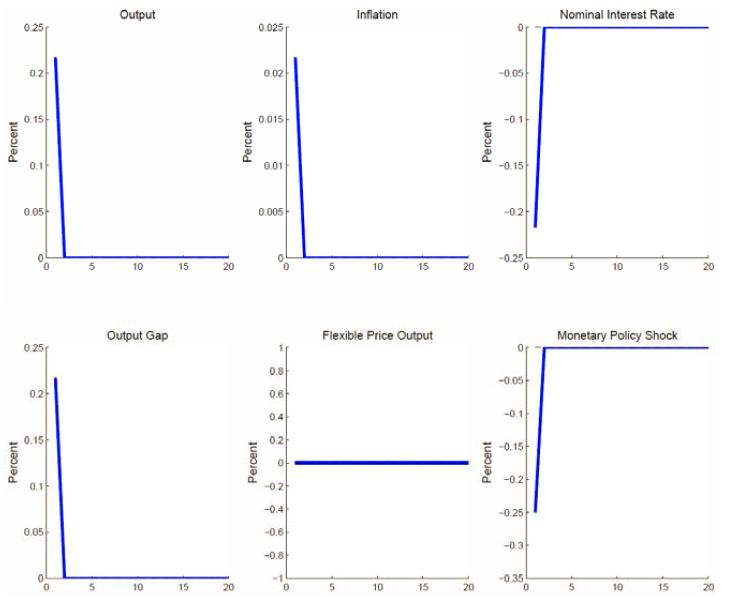
\includegraphics[scale=0.5]{images/moneyshock3DNK}
\end{center}

In conclusion, we can see that money shocks have no real effects, have no lasting effects (only on impact) and no hump-shaped responses (as in our VAR estimates): they describe the reality pretty poorly as is. Nevertheless, we can add elements to the model so that we have better effects. For example, we could imagine that interest rates take time to adjust (not hard to believe considering actual behavior of the FED), we call this phenomenon interest rate smoothing. The effects are of course in the same directions but we see a longer persistence in these effects.\begin{center}
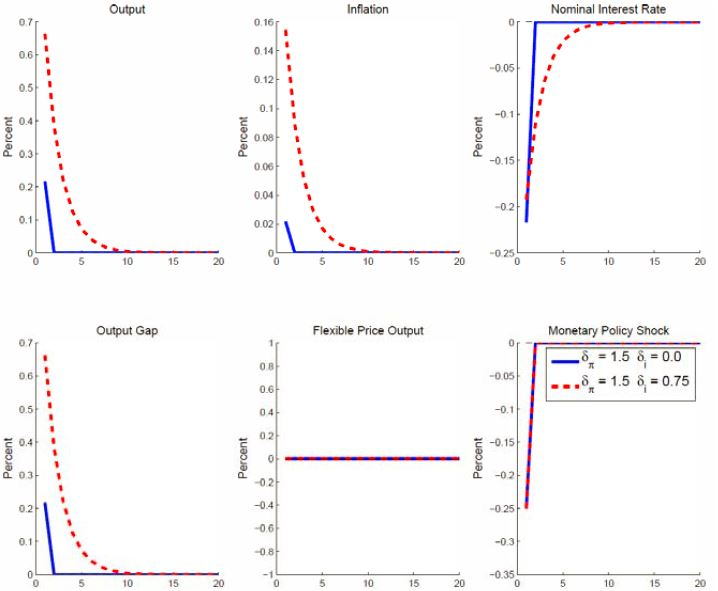
\includegraphics[scale=0.5]{images/moneyshock3DNKi}
\end{center}

\subsubsection{Technology shock}

Now considering a shock to technology, we should see an increase in output with flexible prices and a smaller increase in current output. Therefore we should also see a decrease in output gap, leading to a decrease in inflation and hence a reaction of the central bank to reduce nominal interest rates. Hours worked will go down as the current output increase is not enough to offset the increase in technology. Real wages should go up.\begin{center}
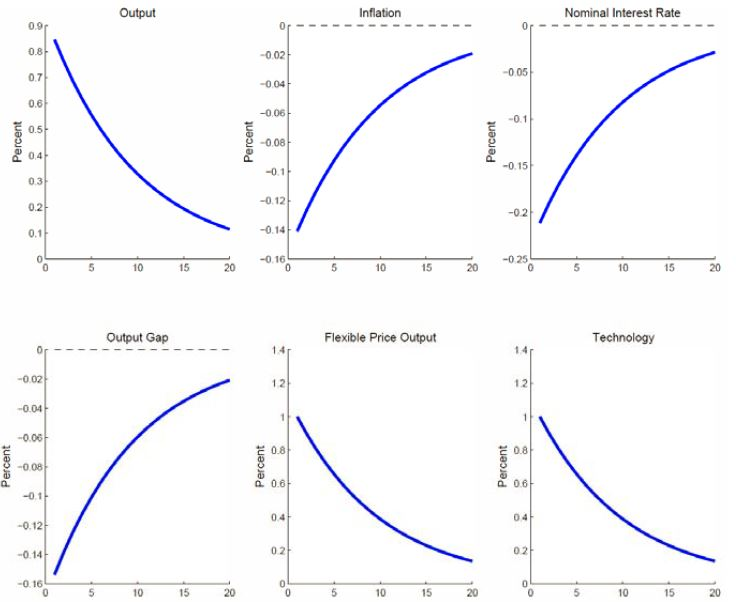
\includegraphics[scale=0.5]{images/techshock3DNK1}
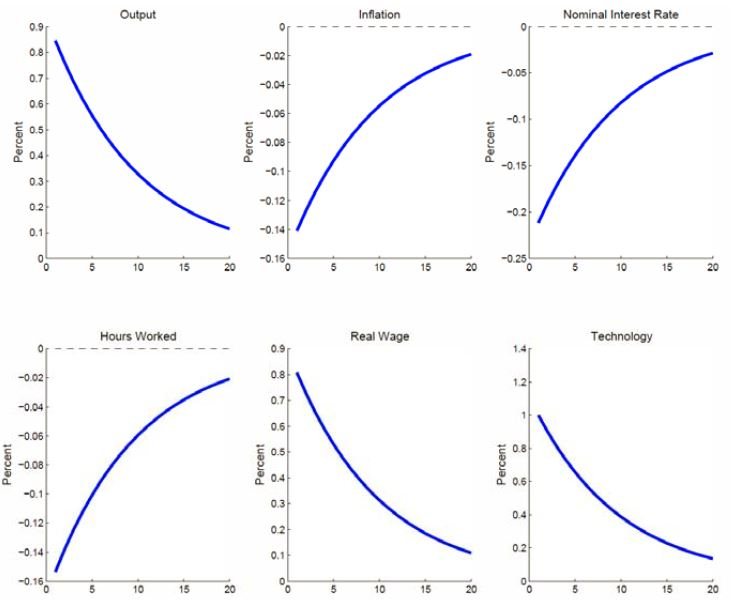
\includegraphics[scale=0.5]{images/techshock3DNK2}
\end{center}

With interest rate smoothing, we get a different story. Indeed, because the interest rate cannot adjust instantly, it is above the optimal interest rate for some time, causing a smaller increase in current output (and a bigger decrease in output gap). This will lead to a lower inflation. Hours worked will decrease more and real wage will increase less.\begin{center}
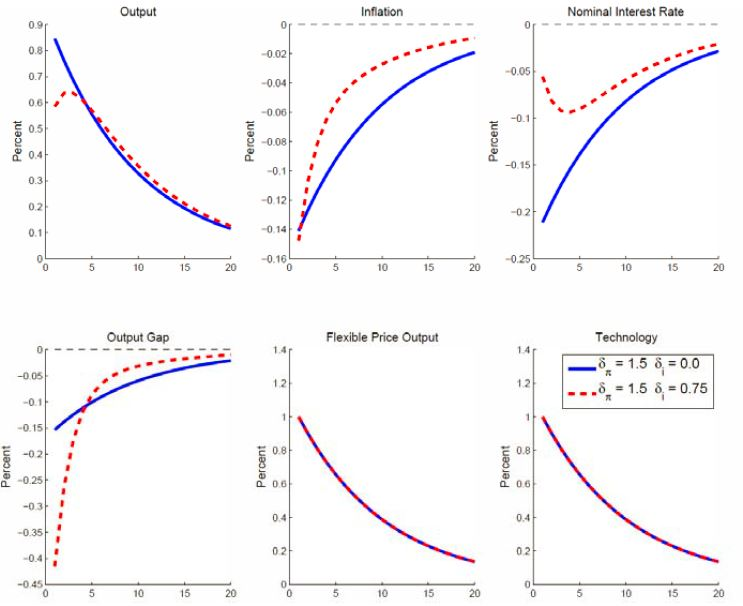
\includegraphics[scale=0.5]{images/techshock3DNK1i}
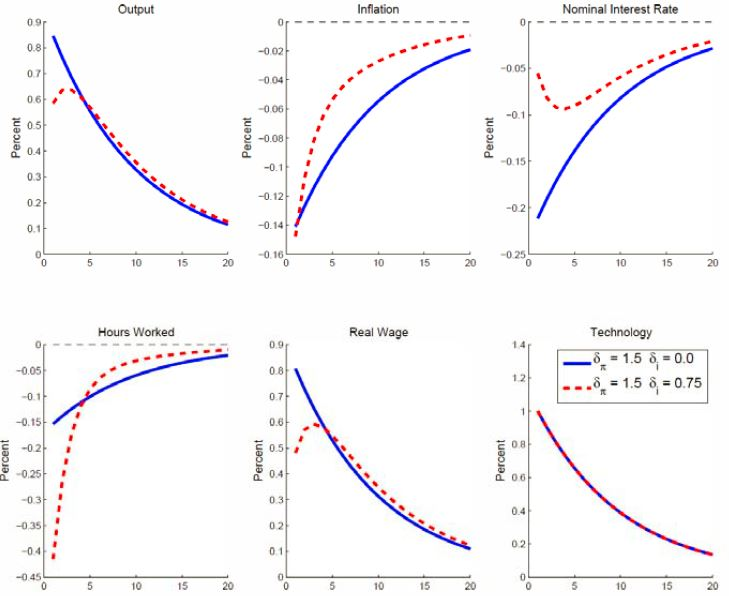
\includegraphics[scale=0.5]{images/techshock3DNK2i}
\end{center}

In conclusion, it seems that while output gaps still exist after a technology shock, the dynamic neo-keynesian model damps it with an active monetary rule. With interest rate smoothing, output gaps are higher (since optimal policy takes longer time to be set). However, this interest rate smoothing appears to create persistent effects and hump-shaped responses, although reducing welfare.

\subsection{Conclusions}

This section has shown that the form of the monetary policy rule has important implications on the dynamics of the economy. In fact, the NK model with exogenous money had no difference in reactions compared to flexible prices. However, a Taylor-rule kind of policy has proven to give different responses, especially with added elements like interest rate smoothing. But this Taylor rule is again an assumption, moreover an assumption that sets the monetary rule at its optimal. How can we make this behaviour depart from optimality?\begin{itemize}
\item We could model a ZLB.
\item We could model the typical way in which interest rates are smoothed.
\item We can add other types of sticky prices (wages, ...).
\end{itemize}

\section{NK model with investment}

This section will give insights as to whether the absence of $I$ and $K$ in our previous model had any impact on the results we found. In order to look at this relationship, we'll analyze the imperfect competition model, adding Calvo frictions in prices. This will yield interesting results, close to what we derived with variable markups but in this model, target markups will not change.

\subsection{Model}

All agents in the economy (consumers, investors and government) demand a composite good $Y_t$ with elasticity of substitution $\sigma$. The demand is: $$Y_t = \left[\int_0^1 y_{it}^\frac{\sigma - 1}{\sigma} \D i\right]^\frac{\sigma}{\sigma - 1} $$ which implies the following demand for each firm $i$ (as derived in the Rotemberg-Woodford model): $$y_{it} = \left(\frac{p_{it}}{P_t}\right)^{-\sigma} Y_t $$

The aggregate production function displays increasing returns to scale (and we'll assume no profit at the steady state, as we did in the Rotemberg-Woodford model), hence: $$Y_t = K_t^\alpha (Z_tH_t)^{1-\alpha} - \Phi $$ which gives the following log-linearized production function:$$ \tilde Y_t = \mu(1 -s_{H})\tilde{K}_t + \mu s_H(\tilde{Z}_t + \tilde{H}_t) $$ where $\mu = \frac{Y^* + \Phi}{Y^*}$ is the degree of returns to scale. In the factor markets, we have: $$R_t = \phi_t\alpha\frac{Y_t + \Phi}{K_t} ; \quad W_t = \phi_t(1 - \alpha)\frac{Y_t + \Phi}{H_t} $$

Adding Calvo prices, we get the following NKPC curve (as derived during the TA session): $$\pi_t = \beta\Et{\pi_{t+1}} + \lambda\tilde \phi_t $$ This time $\tilde\phi_t$ takes a different form because of imperfect competition. From the labor demand FOC, we have: \begin{align*}
\tilde W_t & = \tilde\phi_t + \frac{Y^*}{Y^* + \Phi} \tilde Y_t - \tilde H_t \\ \Leftrightarrow \tilde\phi_t & =\tilde W_t  +\tilde H_t  - \frac{Y^*}{Y^* + \Phi} \tilde Y_t \\ \Leftrightarrow \tilde\phi_t & = \tilde W_t  + \tilde H_t - \tilde Y_t + \tilde Y_t - \frac{Y^*}{Y^* + \Phi} \tilde Y_t \\
\Leftrightarrow \tilde\phi_t & = \tilde s_t^H + \frac{\Phi}{Y^* + \Phi} \tilde Y_t
\end{align*}

We introduce two types of monetary policies: one exogenous, the other is a Taylor-rule with interest rate smoothing. \begin{align*} 
\text{ Exog. Money : } & \tilde M_t - \tilde P_t = \gamma \tilde Y_t - \nu (\tilde r_t + \Et{\pi_{t+1}}) \\ 
\text{ Taylor Rule : } & \tilde i_t = \delta_i \tilde i_{t-1} + \delta_\pi \pi_t + \delta_X \tilde X_t + \varepsilon_t
\end{align*}

Consumers' behavior is unchanged from our usual assumptions in all but one way: they can invest in capital as well as risk-less bonds. This gives a purpose to having two Euler equation: \begin{align*} 
\text{ Euler eq. for bonds: } & \tilde \lambda_{t} =  \beta r^*\cdot \tilde r_{t+1} + \Et{\tilde\lambda_{t+1}} \\ 
\text{ Euler eq. for capital: } & \tilde \lambda_{t} =  \beta R^*\cdot \Et{\tilde R_{t+1}} + \Et{\tilde\lambda_{t+1}}
\end{align*} which means that by the arbitrage condition, it must be that $$r^*\cdot \tilde r_{t+1} = R^*\cdot \Et{\tilde R_{t+1}} \Leftrightarrow \tilde r_{t+1} = \frac{R^*}{r^*} \cdot \Et{\tilde R_{t+1}} = \frac{r^* + \delta}{r^*} \cdot \Et{\tilde R_{t+1}} $$ This last equation is the condition for equilibrium in the assets market. Assuming that $\Et{\tilde R_{t+1}} = \tilde R_{t+1}$ can simplify greatly the graphical analysis adding two interpretations to the model: there's no uncertainty about interest rates, all shocks on interest rates are anticipated. From both factor demand equations we can write: $$\frac{R_t}{W_t} = \frac{\alpha}{1 - \alpha}\frac{H_t}{K_t} \Leftrightarrow \tilde R_t = \tilde W_t + \tilde H_t - \tilde K_t $$ and hence we can write: $$\tilde r_t = \frac{r^* + \delta}{r^*} [\tilde W_t + \tilde H_t - \tilde K_t] $$ This equation is the NRR curve. We can note that this implies that $\tilde r_t$ is increasing in $Y$.

\begin{minipage}{0.34\textwidth}
Graphically, the NRR curve and the LM curve (exogenous money) gives the following relationship, where NRR is the curve in this model, compared to NK the classical NKIS curve from previous models.
\end{minipage}
\begin{minipage}{0.64\textwidth}
\centering
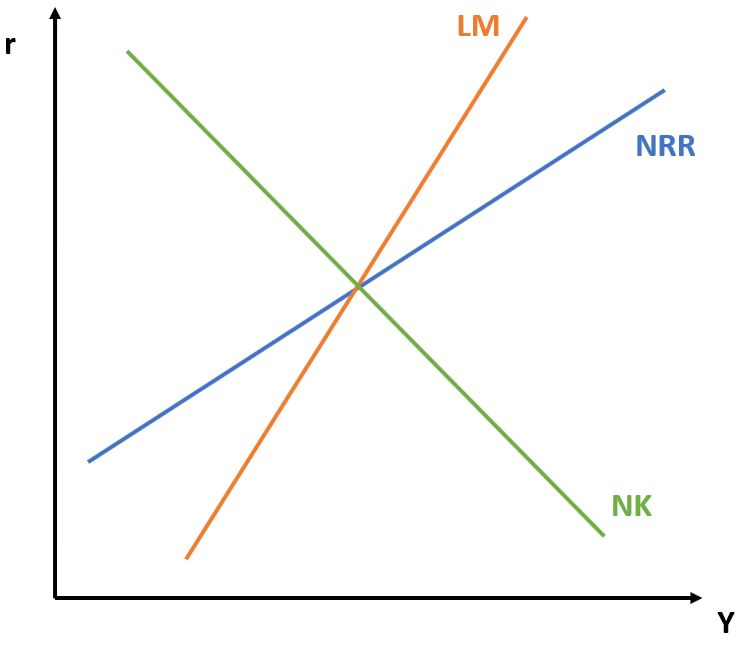
\includegraphics[scale=0.35]{images/graphDNKK}
\end{minipage} \hfill

\subsection{IRFs for NKK models}

\subsubsection{Money supply shocks}

As can be made clear by the previous schematic graph, an increase in the money supply, or a shift to the right of the LM curve, will create an increase in both real interest rates and output. This will in turn cause a decrease in markups, leading to a


\subsubsection{Technology and Government expenditures shocks}





\end{document}